\chapter{TCP拥塞控制}
\minitoc

\section{引言}
本章将探讨 TCP 实现拥塞控制的方法,这也是批量数据传输中最重要的。拥塞控制是TCP 通信的每一方需要执行的一系列行为。这些行为由特定算法规定,用于防止网络因为大
规模的通信负载而瘫痪。其基本方法是当有理由认为网络即将进入拥塞状态(或者已经由于拥塞而出现路由器丢包情况)时减绥 TCP传输。TCP 拥塞控制的难点在于怎样准确地判断何
时需要减缓且如何减缓 TCP 传输,以及何时恢复其原有的速度。

TCP 是提供系统间数据可靠传输服务的协议。第15章已经提到,当 TCP 通信的接收方的接收速度无法匹配发送速度时,发送方会降低发送速度。TCP 的流量控制机制完成了对发
送速率的调节,它是基于 ACK 数据包中的通告窗口大小字段来实现的。这种方式提供了明确的接收方返回的状态信息,避免接收方缓存溢出。

当网络中大量的发送方和接收方被要求承担超负荷的通信任务时,可以考虑采取降低发送速率或者最终丢弃部分数据(也可将两者结合使用)的方法。这是将排队理论应用于路由
器的基本观测结果:即使路由器能够存储一些数据,但若源源不断的数据到达速率高于发出速率,任何容量的中间存储都会溢出。简言之,当某一路由器在单位时间内接收到的数据量
多于其可发送的数据量时,它就需要把多余的部分存储起来。假如这种状况持续,最终存储资源将会耗尽,路由器因此只能丢弃部分数据。

路由器因无法处理高速率到达的流量而被迫丢弃数据信息的现象称为拥塞。当路由器处于上述状态时,我们就说出现了拥塞。即使仅有一条通信连接,也可能造成一个甚至多个路
由器拥塞。若不采取对策,网络性能将大受影响以致瘫痪。在最坏情况下,甚至形成拥塞崩溃。为避免或者在一定程度上缓解这种状况,TCP 通信的每一方实行拥塞控制机制。不同的
TCP 版本(包括运行 TCP/IP 协议栈的操作系统)采取的规程和行为有所差异。本章将着重讨论最常用的方法。
\subsection{TCP 拥塞检测}
如前所述,针对丢包情况,TCP 采取的首要机制是重传,包括超时重传和快速重传(参见第14 章)。考虑如下情形,当网络处于拥塞崩溃状态时,共用一条网络传输路径的多个
TCP 连接却需要重传更多的数据包。这就好比火上浇油,可想而知,结果只会更糟,所以这种情况应该尽量避免。

当拥塞状况出现(或将要出现)时,我们可以减缓 TCP 发送端的发送速率;若拥塞情况有所缓解,可以检测和使用新的可用带宽。然而这在互联网中却很难做到,因为对于TCP
发送方来说,没有一个精确的方法去知晓中间路由器的状态。换言之,没有一个明确的信号告知拥塞状况已发生。典型的TCP 只有在断定拥塞发生的情况下,才会采取相应的行动。
推断是否出现拥塞,通常看是否有丢包情况发生。在TCP 中,丢包也被用作判断拥塞发生与否的指标,用来衡量是否实施相应的响应措施(即以某种方式减级发送)。从20世纪80年
代起,TCP 就一直沿用这种方法。其他拥塞探测方法,包括时延测量和显式拥塞通知(ECN,16.11 节会讨论),使得 TCP能在丢包发生前检测拥塞。在学习一些“经典”算法后,我们将
讨论上述探测方法。

\begin{tcolorbox}
    在当今的有线网络中,出现在路由器或交换机中的拥塞是造成丟包的主要原因。而在无线网络中,传输和接收错误是导致丟包的重要因素。从20世纪90年代
    中期无线网络荻得广泛应用开始,判断丢包是由于拥塞引起还是传输错误引起,一直是研究的热点问题。
\end{tcolorbox}

在第14章中,我们已经看到 TCP 如何利用计时器、确认以及选择确认机制来检测丢包和恢复传输。当有丢包情况出现时,TCP的任务是重传这些数据包。现在我们关心的是,当
观测到丢包后,TCP还做了哪些工作,特别是它如何识别这就是已出现拥塞的信号,进而需要执行减速操作。下面的章节主要讨论 TCP 何时减速以及怎样减速(包括如何恢复传输速
度)。我们首先介绍 TCP 在建立新连接时如何确立基本数据传输速率,以及稳定执行大数据量传输操作的经典算法。另外,我们也整合了近年来对这些算法的研究和改进成果,并细查
了相关扩展资料。在此基础上,我们讨论总结了 TCP 拥塞控制安全和其他相关问题。拥塞控制是网络研究领域的热点[RFC6077],每年都会有相关论文发表。

\subsection{减缓TCP发送}
一个亟待解决的问题是,如何减缓TCP发送。在第15章已经提到,根据接收方剩余缓存空间大小,在TCP 头部设置了通知窗口大小字段,该数值是 TCP 发送方调节发送速率的
依据。进一步说,当接收速率或网络传输速率过慢时,我们需要降低发送速率。实现上述操作,基于对网络传输能力的估计,可以在发送端引入一个窗口控制变量,确保发送窗口大
小不超过接收端接收能力和网络传输能力,即TCP发送端的发送速率等于接收速率和传输速率两者中较小值。

反映网络传输能力的变量称为拥塞窗口(congestion window),记作cwnd。因此,发送端实际(可用)窗口 W就是接收端通知窗口 awnd 和拥塞窗口cwnd 的较小者:

\begin{equation}
    W = min (cwnd, awnd)
\end{equation}

根据上述等式,TCP发送端发送的数据中,还没有收到ACK 回复的数据量不能多于P(以包或字节为单位)。这种已经发出但还未经确认的数据量大小有时称为在外数据值(flight
size),它总是小于等于 W。通常,W可以以包或字节为单位。

\begin{tcolorbox}
    当TCP 不使用选择确认机制时,W的限制作用体现为,发送方发送的报文段序列号不能大于ACK号的最大值与 W之和。而对采用选择确认的发送方则有所
    不同,W被用来限制在外数据值。
\end{tcolorbox}

这看似合乎逻辑,但实际并非如此。因为网络和接收端状况会随时间变化,相应地,awnd 和cwnd 的数值也会随之改变。另外,由于缺少显示拥塞的明确信号(参见前述章节),
TCP发送方无法直接获得cwnd 的“准确”值。因此,变量W、cwnd、awnd 的值都要根据经验设定并需动态调节。此外,如前所述,P的值不能过大或过小—一我们希望其接近带宽
延迟积(Bandwidth-Delay Product, BDP),也称作最佳窗口大小(optimal window size)。W反映网络中可存储的待发送数据量大小,其计算值等于 RTT 与链路中最小通行速率(即发
送端与接收端传输路径中的“瓶颈”)的乘积。逼常的策略是,为使网络资源得到高效利用,应保证在网络申传输的数据量达到BDP。但若在传偷数据值远高于BDP时,会引人不必要
的延时(参见16.10节),所以这也是不可取的。在网络中如何确定一个连接的BDP是难点,需要考虑诸多因素,如路由、时延、统计复用(即共用传倫资派)水平随时间的变化性等。

\begin{tcolorbox}
    这里我们主要讨论由TCP 发送方的数据发送而产生的拥塞,但也要注意因接收方回复ACK而产生的相反方向链路上的删塞,目前也有相关研究针对孩一问
    题。在文献TRFC5690]中介绍了一种方法,该方法中TCP接收方需要很据一定比率国复ACK(即接收了多少个数据包后才能发送一个ACK)。
\end{tcolorbox}

\section{一些经典算法}
当一个新的TCP连接建立之初,还无法知获可用的传输资源,所以cwnd 的初始值也无法确定。(也有一些例外,如有些系统的缓存容量是预先设定的,在第14 章我们称其为目
的度量(destination metrie)。)TCP 通过与接收端交换一个数据包就能获得awnd 的值,不需要任何明确的信号。显而易见,获得cwnd 最佳值的唯一方法是以越来越快的速率不断发送
数据,直到出现数据包丢失(或网络阻塞)为止。这时考虑立即以可用的最大速率发送(受awnd 的限制),或是慢速启动发送。由于多个 TCP 连接共享一个网络传输路径,以全速启动
会影响其他连接的传输性能,所以通常会有特定的算法来避免过快启动,直至稳定传输后才会运行相应的其他算法。

TCP 发送方的拥塞控制操作是由ACK 的接收来驱动或“控制”的。当 TCP 传输处于稳定阶段(cwnd 取合适值),接收到 ACK 回复表明发送的数据包已被成功接收,因此可以继续
发送操作。据此推理,稳定状态下的 TCP抑塞行为,实际是试图使在网络传输路径上的数据包守恒(参见图 16-1)。这里的守恒是从物理学意义上而言的——某个量(如动量、能量)
进入一个系统不会凭室消失或出现,而是以某种表现形式继续存在。

\begin{figure}[!htb]
    \centering
	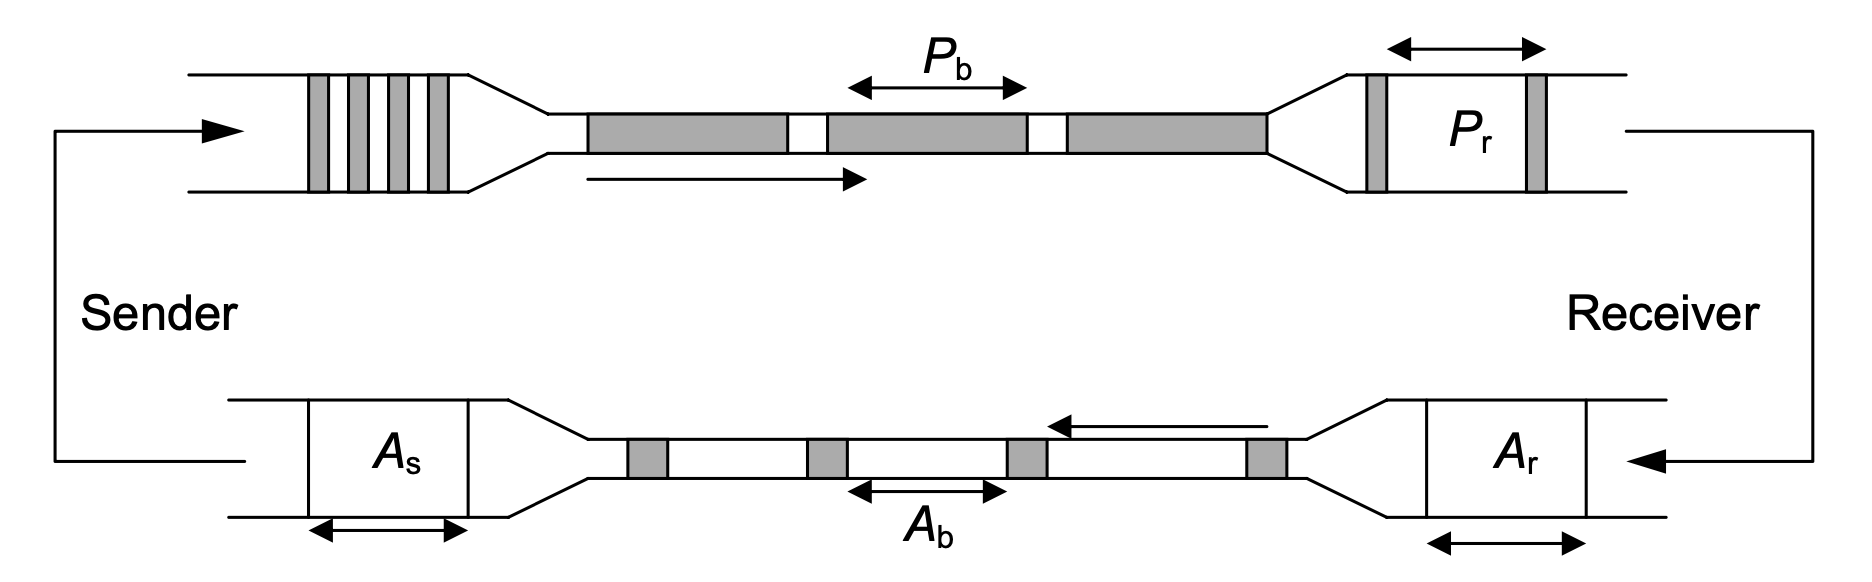
\includegraphics[width=1\textwidth]{imgs/16/16-1.png}
	\caption{TCP拥塞控制操作是基于数据包守恒原理运行的由子传输能力有限,数据包(P)会适时地“伸展”。接收方以一定问隔(P)接收到数据包后,会陆续(以4,为间隔)生成相应的
    ACK,以一定的发送间隔(小)返回给发送方。当ACK 陆线(以A.为间隔)到达发送端时,其到达提供了一个信号或者说“ACK 时钟”,表明发送嘴可以继续发送数帮。在稳定传输状
    态下,整个系统可“自同步"控制(本图改编自 [I88],源丁S. Seshan' s CMU Leeture Notes,2005.3.22)}
\end{figure}

如图16-1 所示,上下两条通道形似“漏汁”。发送方发送的(校大)数擔包经上通道传输给接收方。相对较狄窄部分表不传输较慢的连接链路,数娜包需要适时地被“伸肥”。两
端部分(位于发送方和接收方)让数据包发送前和接收后的队列。下通道传输相应ACK数据包。在高效传输的稳定状态下,上下通道都不会出现包堵塞的情况,而且在上通道中也不会
有较大传输间隔。注意到发送方接收到一个 ACK 就表明可向图16-1 中的上层通道发送一个数据包(即网络中可容纳另一个包)。这种由一个 ACK 到达(称作 ACK 时钟)触发一个新数
据包传输的关系称为自同步(sclf-clocking)。

现在我们讨论 TCP 的两个核心算法:慢启动和拥塞避免。这两个算法是基于包守恒和ACK 时钟原理,最早在 Jacobson [J88]的经典论文里被正式提出。几年后,Jacobson 对拥塞
避免算法提出了改进[J90]。这两个算法不是同时运行的—一在任一给定时刻,TCP 只运行一个算法,但两者可以相互切换。下面我们将详细讨论这两个算法,包括如何使用以及对算
法的改进。每个 TCP连接都能独立运行这两个算法。

\subsection{慢启动}
当一个新的TCP 连接建立或检测到由重传超时(RTO)导致的丢包时,需要执行慢启动。TCP 发送端长时间处于空闲状态也可能调用慢启动算法。慢启动的目的是,使TCP 在
用拥塞避免探寻更多可用带宽之前得到cwnd值,以及帮助TCP建立ACK 时钟。通常,TCP 在建立新连接时执行慢启动,直至有丢包时,执行拥塞避免算法(参见16.2.2节)进入
稳定状态。下文引自 [RFC5681]:

在传输初始阶段,由于未知网络传输能力,需要缓慢探测可用传输资源,防止短时间内大量数据注入导致拥塞。慢启动算法正是针对这一问题而设计。在数据传
输之初或者重传计时器检测到丢包后,需要执行慢启动。

TCP 以发送一定数目的数据段开始慢启动(在SYN交换之后),称为初始窗口(InitialWindow, IW)。IW 的值初始设 一个 SMSS(发送方的最大段大小),但在[RFCS681]中设
为一个稍大的值,计算公式如下:

\begin{equation}
    IW =2* (SMSS)且小于等于2个数据段(当SMSS>2190字节)
    IW =3* (SMSS)且小于等于3个数据段(当2190≥SMSS>1095字节)
    IW =4*(SMSS)且小于等于4个数据段(其他)
\end{equation}

上述 IW的计算方式可能使得初始窗口为几个数据包大小(如3个或4个),为简单起见,我们只讨论IW =1 SMSS 的情况。TCP 连接初始的cwnd =1 SMSS,意味着初始可用
窗口W也为1 SMSS。注意到大部分情况下,SMSS 为接收方的 MSS(最大段大小)和路径MTU(最大传输单元)两者中较小值。

假设没有出现丢包情况且每个数据包都有相应的ACK,第一个数据段的ACK 到达,说明可发送一个新的数据段。每接收到一个好的ACK 响应,慢启动算法会以 min (N, SMSS)
来增加 cwnd值。这里的N 是指在未经确认的传输数据中能通过这一“好的ACK”确认的字节数。所谓的“好的ACK”是指新接收的 ACK 号大于之前收到的ACK。

\begin{tcolorbox}
    已被 ACK 确认的字节数目用于支持适当字节计数(Appropriate Byte Counting,ABC)[RFC3465],这是[RFC5681]推荐的实验规范。ABC 用于计数“ACK 分裂”
    攻击(将在16.12 节叙述),指利用许多较小ACK使TCP 发送方加速发送。Linux 利用布尔系统配置变量 \verb|net.ipv4.tep_abe| 设定 ABC是否可用(默认不可用)。在最近的
    几个 Windows 版本中,ABC默认开启。
\end{tcolorbox}

因此,在接收到一个数据段的ACK后,通常 cwnd 值会增加到2,接着会发送两个数据段。如果成功收到相应的新的 ACK,cwnd 会由2变4,由4变8,以此类推。一般情况下,
假设没有丢包且每个数据包都有相应 ACK,在k轮后W的值为W=2’,即k=10g2W,需要K个 RTT 时间操作窗口才能达到 W大小。这种增长看似很快(以指数函数增长),但若与一
开始就允许以最大可用速率(即接收方通知窗口大小)发送相比,仍显缓慢。(W不会超过awnd。)

如果假设某个 TCP 连接中接收方的通知窗口非常大(比如说,无穷大),这时 cwnd 就是影响发送速率的主要因素(设发送方有较大发送需求)。如前所述,cwnd 会随着 RTT 呈指数
增长。因此,最终 cwnd(W也如此)会增至很大,大量数据包的发送将导致网络瘫痪(TCP吞吐量与 W/RTT 成正比)。当发生上述情况时,cwnd 将大幅度减小(减至原值一半)。这是
TCP 由慢启动阶段至拥塞避免阶段的转折点,与cwnd 和慢启动圖值(slow start threshold,ssthresh)相关。

图16-2(左)描述了慢启动操作。数值部分以 RTT 为单位。假设该连接首先发送一个包(图上部),返回一个 ACK,接着在第二个 RTT 时间里发送两个包,会接收到两个ACK。
TCP 发送方每接收一个ACK 就会执行一次cwnd 的增长操作,以此类推。右图描述了 cwnd随时间增长的指数函数。图中另一条曲线显示了每两个数据包收到一个ACK 时 cwnd 的增长
情况。通常在 ACK 延时情况下会采用这种方式,这时的 cwnd 仍以指数增长,只是增幅不是很大。正因 ACK 可能会延时到达,所以一些 TCP 操作只在慢启动阶段完成后才返回ACK。
Linux 系统中,这被称为快速确认(“快速 ACK 模式”),从内核版本2.4.4开始,快速确认一直是基本 TCP/P 协议栈的一部分。

\begin{figure}[!htb]
    \centering
	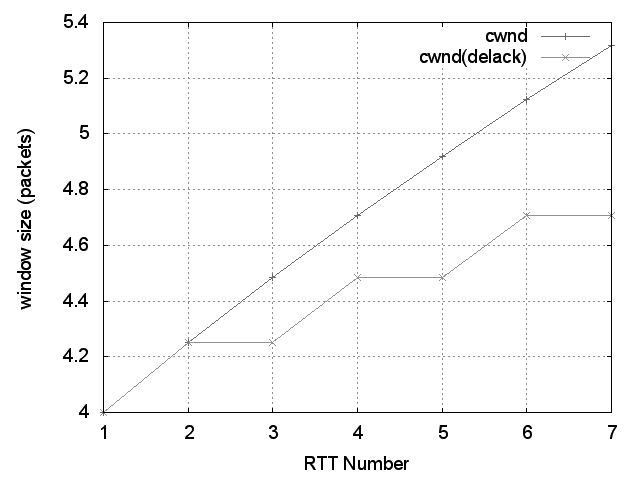
\includegraphics[width=0.7\textwidth]{imgs/16/16-3.png}
	\caption{经典慢启动算法操作。在没有 ACK 延时情况下,每接收到一个好的ACK 就意味着发送方可以发送两个新的数据包(左)。这会使得发送方窗口随时间垦指数增长(右,上方曲线)。当发生
    ACK 延时,如每脂一个數据包生成一个ACK, cwnd 仍3以、指数增长,但增幅较小(右,下方曲线)}
\end{figure}

\subsubsection{拥塞避免}
如上所述,在连接建立之初以及由超时判定丢包发生的情况下,需要执行慢肩动操作。在慢启动阶段,cwnd 会快速增长,帮助确立一个慢启动阈值。一旦达到阈值,就意味着可
能有更多可用的传输资源。如果立即全部占用这些资源,将会使共享路由器队列的其他连接出现严重的丢包和重传情况,从而导致整个网络性能不稳定。

为了得到更多的传输资源而不致影响其他连接传输,TCP 实现了拥塞避免算法。一旦确立慢启动阈值,TCP 会进入拥塞避免阶段,cwnd 每次的增长值近似于成功传输的数据段大小。
这种随时间线性增长方式与慢启动的指数增长相比级慢许多。更准确地说,每接收一个新的ACK, cwnd 会做以下更新:
\begin{equation}
    cwnd, + 1 = cwnd, + SMSS * SMSS/cwnd,
\end{equation}

分析上式,假设 cwndo =k*SMSS 字节分k段发送,在接收到第一个ACK后,cwnd 的值增长了 1/k倍:
\begin{equation}
    cwnd, = cwndo + SMSS*SMSS/cwndo = k*SMSS + SMSS * (SMSS/ (k * SMSS) )
= k * SMSS + (1/k) *SMSS = (k + (1/k)) *SMSS = cwndo + (1/k) *SMSS
\end{equation}

随着每个新的ACK 到达,cwnd 会有相应的小幅增长(取决于上式中的k值),整体增长率呈现轻微的次线性。尽管如此,我们通常认为拥塞避免阶段的窗口随时间线性增长(见
图 16-3),而慢启动阶段呈指数增长(见图16-2)。这个函数也称为累加增长,因为每成功接收到相应数据,cwnd 就会增加一个特定值(这里大约是一个包大小)。

\begin{figure}[!htb]
    \centering
	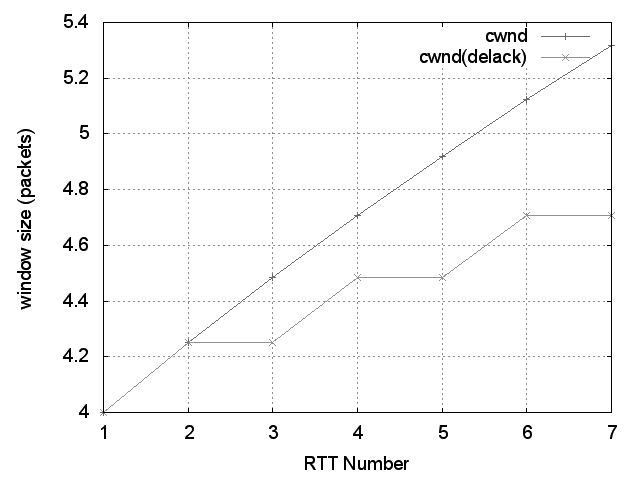
\includegraphics[width=0.7\textwidth]{imgs/16/16-3.png}
	\caption{拥塞避免算法操作。若没有 ACK延时发生,每接收一个好的ACK,就意味着发送方可继续发送1/W个新的数据包。发送窗口随时间近似呈线性增长(右,上方曲线)。当有ACK 延时,
    如每隔一个数据包生成一个 ACK,cwnd 仍近似星线性增长,只是增幅较小(右,下方曲线)}
\end{figure}

图16-3(左)描述了拥塞避免操作。数值部分仍是以 RTT为单位。假设连接发送了4个数据包(图上方),返回了4个ACK,cwnd 可以有相应的增长。在第2个RTT阶段,增长
可达到整数值,使得cwnd增加一个 SMSS,这样可以继续发送一个新的数据包。右图描绘了cwnd 随时间近似呈线性增长。另一曲线模拟 ACK 延时,显示了每两个数据包收到一个
ACK 时cwnd 的增长情况。这时的cwnd仍近似呈线性增长,只是增幅不是很大。

拥塞避免算法假设由比特错误导致包丢失的概率很小(远小于1\%),因此有丢包发生就表明从源端到目的端必有某处出现了拥塞。如果假设不成立,比如在无线网络中,那么即使
没有拥塞 TCP传输也会变慢。另外,cwnd的增大可能会经历多个 RTT,这就需要有充裕的网络资源,并得到高效利用。这些问题还有很大的研究空间,以后我们将会讨论其中一些方法。

\subsection{慢启动和拥塞避免的选择}
在通常操作中,某个 TCP连接总是选择运行慢启动和拥塞避免中的一个,不会出现两者同时进行的情况。现在我们考虑,在任一给定时刻如何决定选用哪种算法。我们已经知
道,慢启动是在连接建立之初以及超时发生时执行的。那么决定使用慢启动还是拥塞避免的关键因素是什么呢?

前面我们已经提到过慢启动阈值。这个值和 cwnd的关系是决定采用慢启动还是拥塞避免的界线。当 cwnd < ssthresh,使用慢启动算法:当 cwnd > ssthresh,需要执行拥塞避免:
而当两者相等时,任何一种算法都可以使用。由上面描述可以得出,慢启动和拥塞避免之间最大的区别在于,当新的ACK 到达时,cwnd怎样增长。有趣的是,慢启动阈值不是固定的,
而是随时间改变的。它的主要目的是,在没有丢包发生的情况下,记住上一次“最好的”操作窗口估计值。换言之,它记录 TCP 最优窗口估计值的下界。

慢启动阈值的初始值可任意设定(如 awnd 或更大),这会使得 TCP 总是以慢启动状态开始传输。当有重传情况发生,无论是超时重传还是快速重传,ssthresh 会按下式改变:
\begin{equation}
    ssthresh = max(在外数据值 /2, 2*SMSS)
\end{equation}
我们已经知道,如果出现重传情况,TCP 会认为操作窗口超出了网络传输能力范围。这时会将慢启动阈值(ssthresh) 减小至当前窗口大小的一半(但不小于 2*SMSS),从而减小最
优窗口估计值。这样通常会导致 ssthresh 减小,但也有可能会使之增大。分析 TCP 拥塞避免的操作流程,如果整个窗口的数据都成功传输,那么cwnd值可以近似增大1 SMSS。因
此,若cwnd 在一段时间范围内已经增大,将 ssthresh 设为整个窗口大小的一半可能使其增大。这种情况发生在当TCP 探测到更多可用带宽时。在慢启动和拥塞避免结合的情况下,
ssthresh 和cwnd 的相互作用使得TCP 拥塞处理行为显现其独有特性。下面我们探讨将两者结合的完整的算法。

\subsection{Tahoe、Reno 以及快速恢复算法}
至此讨论的慢启动和拥塞避免算法,组成了 TCP 拥塞控制算法的第一部分。它们于20世纪80年代末期在加州大学伯克利分校的4.2版本的UNIX 系统中被提出,称为伯克利软件
版本,或BSD UNIX。至此开始了以美国城市名命名各个 TCP版本的习惯,尤其是那些赌博合法的城市。

4.2版本的BSD(称为 Tahoe)包含了一个TCP版本,它在连接之初处于慢启动阶段,若检测到丢包,不论由于超时还是快速重传,都会重新进入慢启动状态。有丢包情况发生
时,Tahoe简单地将 cwnd 减 初始值(当时设为1 SMSS)以达到慢启动目的,直至ewnd增长为 ssthresh。

这种方法带来的一个问题是,对于有较大BDP的链路来说,会使得带宽利用率低下。因为TCP 发送方经重新慢启动,回归到的还是未丢包状态(cwnd 启动初始值设置过小)。
为解决这一问题,针对不同的丢包情况,重新考虑是否需要重回慢启动状态。若是由重复ACK 引起的丢包(引发快速重传),cwnd 值将被设为上一个 ssthresh,而非先前的1 SMSS。
(在大多数 TCP 版本中,超时仍是引发慢启动的主要原因。)这种方法使得TCP 无须重新慢启动,而只要把传输速率减半即可。

进一步讨论较大BDP链路的情况,结合之前提到的包守恒原理,我们可以得出结论,只要接收到 ACK 回复(包括重传 ACK),就有可能传输新的数据包。BSD UNIX 的4.3 BSD
Reno版中的快速恢复机制就是基于上述结论。在恢复阶段,每收到一个 ACK,cwnd 就能(临时)增长1 SMSS,相应地就意味着能发送一个新的数据包。因此拥塞窗口在一段时间内
会急速增长,直到接收一个好的ACK。不重复的(“好的”)ACK 表明 TCP 结束恢复阶段,拥塞已减少到之前状态。TCP Reno 算法得到了广泛应用,并成为“标准 TCP”的基础。

\subsection{标准 TCP}
尽管究竟哪些构成了“标准”TCP还存在争议,但我们讨论过的上述算法毋庸置疑都属于标准 TCP。慢启动和拥塞避免算法通常结合使用,[RFC5681]给出了其基本方法。这个规
范并不要求严格使用这些精确算法,TCP 实现过程仅利用其核心思想。

总结[RFC5681]中的结合算法,在TCP 连接建立之初首先是慢启动阶段(cwnd =IW),ssthresh 通常取一较大值(至少为 awnd)。当接收到一个好的ACK(表明新的数据传输成功),
cwnd 会相应更新:

\begin{equation}
    cwnd += SMSS(若 cwnd < ssthresh)慢启动
    cwnd += SMSS*SMSS/cwnd(若 cwnd>ssthresh)拥塞避免
\end{equation}

当收到三次重复 ACK(或其他表明需要快速重传的信号)时,会执行以下行为:
\begin{enumerate}
    \item ssthresh 更新为大于等式(16-1)中的值。
    \item 启用快速重传算法,将 cwnd 设为(ssthresh +3*SMSS)。
    \item 每接收一个重复 ACK,cwnd 值暂时增加1 SMSS。
    \item 当接收到一个好的ACK,将 cwnd 重设力 ssthresh。
\end{enumerate}

以上第2步和第3步构成了快速恢复。步骤2设置cwnd 大小,首先cwnd 通常会被减为之前值的一半。然后,考虑到每接收一个重复 ACK,就意味着相应的数据包已成功传输
(因此新的数据包就有发送机会),cwnd 值会相应地暂时增大。这一步也可能出现cwnd 加速递减的情况,因为通常 cwnd 会乘以某个值(这里取0.5)来形成新的cwnd。步骤3维持
cwnd 的增大过程,使得发送方可以继续发送新的数据包(在不超过 awnd 的情况下)。步骤4假设 TCP 已完成恢复阶段,所以 ewnd 的临时膨胀也消除了(有时称这一步为“收缩”)。

以下两种情况总会执行慢启动:新连接的建立以及出现重传超时。当发送方长时间处于空闲状态,或者有理由怀疑 cwnd 不能精确反映网络当前拥塞状态(参见16.3.5节)时,也可
能引发慢启动。在这种情况下,cwnd 的初始值将被设为重启窗口(RW)。在文献[RFC5681]中,推荐 RW值为RW=min (IW,cwnd)。其他情况下,慢启动中ownd 初始设为IW。

\section{对标准算法的改进}
经典的标准 TCP 算法在传输控制领域做出了重大贡献,尤其针对网络拥塞崩溃这一难题,取得了显著效果。

\begin{tcolorbox}
    在1986~1988年,网络胡塞崩溃是引起广泛关注的难点问题。1986年10月,作为早期互联网的重要组成部分,NSFNET 主干网出现了一次严亚故障,运行速度
    仅为其应有速度的千分之十(称力 “NSFNET 危机”)。问题的主要形成原因在于对大量的重传没有任何控制操作。持续的拥塞状态导致了亚严重的丢包现象(由于更
    多的重传操作)和吞吐量低下。采用经典拥塞控制算法有效地解决了这一问题。
\end{tcolorbox}


然而,仍然可以找到值得改进的地方。考虑到 TCP 的普遍使用性,越来越多的研究致力于使TCP 在更广泛的环境里更好地工作。下面我们提出几种方法,现在许多 TCP版本也
已经实现。

\subsection{NewReno}
快速恢复带来的一个问题是,当一个传输窗口出现多个数据包丢失时,一旦其中一个包重传成功,发送方就会接收到一个好的 ACK,这样快速恢复阶段中cwnd 窗口的暂时膨胀就
会停止,而事实上丢失的其他数据包可能并未完成重传。导致出现这种状况的ACK 称为局部ACK(partial ACK)。Reno算法在接收到局部 ACK 后就停止拥塞窗口膨胀阶段,并将其
减小至特定值,这种做法可能导致在重传计时器超时之前,传输通道一直处于空闲状态。力理解出现这种情况的原因,我们首先明确,TCP(无选择确认机制)需要通过三个(或重复
阈值)重复 ACK 包作为信号才能触发快速重传机制。假如网络中没有足够的数据包在传输,那么就不可能因丢包而触发快速重传,最终导致重传计时器超时,引发慢启动操作,从而严
重影响网络吞吐性能。

为解决上述问题,[RFC3782]提出了一种改进算法,称为NewReno。该算法对快速恢复做出了改进,它记录了上一个数据传输窗口的最高序列号(即我们在第14章提到的恢复点)。
仅当接收到序列号不小于恢复点的ACK,才停止快速恢复阶段。这样 TCP 发送方每接收一个ACK 后就能继续发送一个新数据段,从而减少重传超时的发生,特别针对一个窗口出现
多个包丢失的情况时。NewReno是现在比较常用的一个 TCP版本,它不会出现经典快速重传的问题,实现起来也没有选择确认(SACK)复杂。然而,当出现上述多个丢包情况时,
利用SACK 机制能比 NewReno获得更好的性能,但需要较为复杂的拥塞控制操作,下面我们会讨论这一问题。

\subsection{采用选择确认机制的TCP拥塞控制}
在TCP 引人SACK 与选择性重复之后,发送方能够更好地确定发送哪个数据段来填补接收方的空缺(参见第14章)。为了填补接收数据的空峡,发送方通常只发送丢失的数据段,
直至完成所有重传。这和前面提到的基本的快速重传/恢复机制有所差别。

在快速重传/恢复情况下,当出现丢包,TCP 发送方只重传它认为已经丢失的包。如果窗口W允许,还可以发送新的数据包。在快速恢复阶段,由于窗口大小会随着每个 ACK的
到达而膨胀,在完成重传后,通常发送方能有更大的窗口发送更多新数据。采用SACK 机制后,发送方可以知晓多个数据段的丢失情况。因为这些数据都在有效窗口内,理论上可
以即时重传。然而,这样可能会在较短时间内向网络中注人大量数据,削弱拥塞控制效果。SACK TCP 会引发以下问题:在恢复阶段,只使用cwnd 作为发送方滑动窗口的界限来表示
发送多少个(以及哪些)数据包是不够的,且选择发送哪些数据包与发送时间紧密相关。换言之,SACK TCP 强调拥塞管理和选择重传机制的分离。传统(无SACK)TCP则将两者结合。

一种实现分离的方法是,除了维护窗口,TCP 还负责记录注入网络的数据量。[RFC3517]称其为管道(pipe)变量,这是对在外数据的估计值。管道变量以字节(或包,依不同实现方
式而定)为单位,记录传输和重传情况(不考虑丢包,将两者同等对待)。假设 awnd 值较大,只要不等式cwnd - pipe ≥ SMSS 成立,在任何时候SACK TCP 均可发送数据。这里cwnd
仍被用来限定可传输至网络中的数据量,但除了窗口本身,网络中数据量的估计值也被记录了。[FF96] 详细分析比较了SACK TCP 和传统 TCP的拥塞控制方法,并做了相关仿真工作。

\subsection{转发确认(FACK)和速率减半}
对基于 Reno(包括 NewReno)的TCP版本来说,当快速重传结束后cwnd 值减小,在TCP发送新数据之前至少可以接收一半已发送数据返回的ACK。这和检测到丢包后立即将
拥塞窗口值减半相一致。这样 TCP发送端在前一半的 RTT时间内处于等待状态,在后一半RTT 才能发送新数据,这是我们不愿看到的。

在丢包后,为避免出现等待空闲而又不违背将拥塞窗口减半的做法,[MM96] 提出了转发确认 (forward acknowledgment,FACK)策略。FACK 包含了两部分算法,称为“过度衰减”
(overdamping)和“缓慢衰减”(rampdown)。从最初想法的提出到改进,最终在Hoe 的工作基础上[H96]形成了统一的算法,称为速率减半(rate halving)。为控制算法尽可能有效地运
行,进一步添加了界定参数,完整的算法被称为带界定参数的速率减半(Rate-Halving withBounding Parameters, RHBP)算法 [PSCRH]。

RHBP 的基本操作是,在一个 RTT 时间内,每接收两个重复ACK,TCP 发送方可发送一个新数据包。这样在恢复阶段结束前,TCP 已经发送了一部分新数据,与之前的所有发送
都挤在后半个 RTT 时间段内相比,数据发送比较均衡。由于过度集中的发送操作可能持续多个 RTT,对路由缓存造成负担,因此均衡发送是比较有利的。

为了记录较为精确的在外数据估计值,RHBP 利用SACK信息决定FACK 策略:已知的最大序列号的数据到达接收方时,在外数据值加1。注意区分即将发送数据的最大序列号
(图15-9中的 SND.NXT),FACK 给出的在外数据估计值不包括重传。

RHBP 中区分了调整间隔(adjustment interval,cwnd 的修正阶段)和恢复间隔(repairinterval,数据重传阶段)。一旦出现丢包或其他拥塞信号就立即进人调整间隔。调整间隔结
束后 cwnd 的最终值为:至检测时间为止,网络中已正确传输的窗口数据量的一半。RHBP要求发送方传输数据需满足下式;
\begin{equation}
    (SND.NXT - fack + retran_ data + len) < cwnd
\end{equation}

上面的等式得到了包括重传的在外数据值,确保当继续发送一个len 长度的新数据,也不会超过cwnd。假设在 FACK之前的数据已经不在网络中(如丢失或被接收),这样cwnd
就能很好地控制SACK发送方的发送。然而由于SACK 的选择确认特性,可能导致数据包的传输次序过度重排。

Linux 系统实现了 FACK 和速率减半,并默认启用。若 SACK 开启,并将布尔配置变量\verb|net.ipv4.tcp_fack| 置1,就会激活 FACK。当检测到网络中出现数据包失序,FACK的进一步
行为将被禁用。

速率减半是调节发送操作或避免集中发送的方法之一。我们已经了解了它的优点,但这种方法仍然存在一些问题。[ASA00]利用仿真的方法,详细分析了 TCP 发送调度,结果显示
在很多情况下,它的性能劣于 TCP Reno。另外,研究表明,在接收窗口限制 TCP 连接的情况下,速率减半方法收效甚微 [MM05]。

\subsection{限制传输}
[RFC3042] 提出了限制传输(Iimited transmit),它对TCP 做出了微小改进,目的在于使TCP能在可用窗口较小的情况下更好工作。之前已经提到,在Reno 算法中,通常需要三次
重复 ACK 表明数据包丢失。在窗口较小的情况下,当出现丢包,网络中可能没有足够的包去引发快速重传/恢复机制。

采用限制传输策略,TCP发送方每接收两个连续的重复 ACK,就能发送一个新数据包。这就使得网络中的数据包维持一定数量——足以触发快速重传。TCP 因此也可以避免长时
间等待 RTO(可能达到几百毫秒,相对时间较长)而导致吞吐性能下降。限制传输已经成为TCP推荐策略。速率减半也是限制传输的一种形式。

\subsection{拥塞窗口校验}
TCP拥塞管理可能会出现一个问题,那就是发送端可能在一段时间内停止发送(由于没有新数据需要发送或者其他原因阻住发送)。通常情况下,发送操作不会暂停。发送端发送
数据,同时接收 ACK 反馈,以此估计一定时间内(一个 RTT)的 cwnd 和 ssthresh。

在发送操作持续一段时间后,cwnd 可能会增至一个较大值。若发送需要暂停(一定时间后会恢复),根据此时cwnd 的值,在暂停前发送方仍可向网络中(高速)注人大量数据。
若暂停时间足够长,之前的cwnd 可能无法准确反映路径中的拥塞状况。

[RFC2861] 提出了一种拥塞窗口校验 (Congestion Window Validation,cwv)机制。在发送长时间暂停的情况下,由ssthresh 维护 cwnd 保存的“记忆”,之后cwnd 值会衰减。为
理解这种机制,需要区分空闲(idle)发送端和应用受限(application-limited)发送端。对空闲发送端而言,没有发送新数据的需求,之前发送的数据也已经成功接收ACK。因此,整
个连接处于空闲状态——除了必要的窗口更新外(参见第15章),没有数据和ACK 的传输。应用受限发送端则需要传输数据,但由于某种原因无法发送(可能由于处理器正忙或者下层
阻住数据发送)。这种情况会导致连接利用率低下,但并非完全空闲,之前已发送数据返回的ACK 仍可传输。

CwV算法原理如下:当需要发送新数据时,首先看距离上次发送操作是否超过一个RTO。如果超过,则

\begin{itemize}
    \item 更新 ssthresh 值—设 max (ssthresh, (3/4) *cwnd)。
    \item 每经一个空闲 RTT 时间,cwnd 值就减半,但不小于1 SMSS。
\end{itemize}
对于应用受限阶段(非空闲阶段),执行相似的操作:
\begin{itemize}
    \item 已使用的窗口大小记为 \verb|W_used|。
    \item 更新 ssthresh 值一—设为 max (ssthresh, (3/4) *cwnd)。
    \item cwnd设力cwnd 和 \verb|W_used| 的平均值。
\end{itemize}

上述操作均减小了cwnd,但 ssthresh 维护了cwnd 的先前值。第一种情况中,如果传输通道长时间空闲,cwnd 将会显著减小。在某些情况下,这种拥塞窗口的处理方法可以取
得更好效果。根据作者的研究,避免空闲阶段可能发生的大数据量注入,可以减轻对有限的路由缓存的压力,从而减少丢包情况的产生。注意到CWV 减小了cwnd值,但没有减小
ssthresh,因此采用这种算法的通常结果是,在长时间发送暂停后,发送方会进入慢启动阶段。Linux TCP 实现了CWV 并默认启用。

\section{伪 RTO 处理——Eifel 响应算法}
在第15章已经提到,若TCP 出现突发的延时,即使没有出现丢包,也可能造成重传超时的假象。这种伪重传现象的发生可能由于链路层的某些变化(如蜂宽转换),也可能是由
于突然出现严重拥塞造成 RTT大幅增长。当出现重传超时,TCP 会调整 ssthresh 并将 cwnd置为IW,从而进人慢启动状态。假如没有出现实际丢包,在RTO 之后到达的ACK 会使得
cwnd快速增大,但在 cwnd 和ssthresh 值重新稳定前,仍然会有不必要的重传,浪费传输资源。

针对上述问题已有相关探测方法。我们在第14章讨论了其中的一些方法(如DSACK、Eifel、F-RTO)。其中任一探测方法只要结合相关响应算法,就能“还原”TCP 对拥塞控
制变量的操作。一种比较常用(即在IETF 标准化过程中)的响应算法就是Eifel 响应算法[RFC4015]。

Eifel 算法包含检测算法和响应算法两部分,两者在理论上是独立的。任何使用 Eifel 响应算法实现的TCP操作,必须使用相应的标准操作规范或实验 RFC(即被记录的RFC)中
规定的检测算法。

Eifel 响应算法用于处理重传计时器以及重传计时器超时后的拥塞控制操作。这里我们只讨论与拥塞相关的响应算法。在首次发生超时重传时,Eifel 算法开始执行。若认为出现伪
重传情况,会撤销对 ssthresh 值的修改。在所有情况下,若因 RTO 而需改变 ssthresh 值,在修改前需要记录一个特殊变量:\verb|pipe_prev = min|(在外数据值,ssthresh)。然后需要运行一
个检测算法(即之前提到的检测方法中的某个)来判断 RTO 是否真实。假如出现伪重传,则当到达一个 ACK 时,执行以下步骤:

\begin{enumerate}
    \item 若接收的是包含ECN-Echo 标志位的好的ACK,停止操作(参见16.11节)。
    \item cwnd =在外数据值+ min (\verb|bytes_acked|, IW)(假设cwnd 以字节为单位)。
    \item ssthresh = \verb|pipe_prevo|
\end{enumerate}

在改变 ssthresh 之前需要设置\verb|pipe_prev| 变量。\verb|pipe_prev| 用于保存ssthresh 的记录值,以便在步骤3中重设 ssthresh。步骤1针对带 ECN 标志位的ACK 的情况(在16.11 节中将详
细讨论 ECN)。这种情况下撤销 ssthresh 修改会引入不安全因素,所以算法终止。步骤2和步骤3是算法的主要部分(针对cwnd)。步骤2将cwnd设置 一定值,允许不超过IW 的新
数据进入传输通道。因为即使在未知链路拥塞与否的状况下,发送IW 的新数据也被认为是安全的。步骤3在真正的 RTO 发生前重置 ssthresh,至此撤销操作完成。

\section{扩展举例}
下面我们通过一个例子来演示一下前面章节提到的操作算法。利用sock 程序,在一条DSL 线路上传输 2.5MB 数据。发送方和接收方分别为 Linux (2.6)和 FreeBSD(5.4)。链
路在发送方向上限速约为300Kb/s。FreeBSD 接收端处于高带宽连接。发送端至接收端的最小 RTT为15.9ms,需经17个跳步。大部分处理操作均使用基础算法(如慢启动和拥塞避
免),以避免不同操作系统的实现细节差异(后面我们会提到相关问题)。下面开始实验,首先在接收端运行如下操作命令:

\begin{verbatim}
    FreeBSD8
sock -1 -r 32768 -R 233016 -8 6666
\end{verbatim}

该命令为sock 程序设置了一个较大的套接字接收级存(228KB),并执行大数据量的读操作(32KB)。对于传输链路来说,接收缓存已足够大。接着设置发送端为发送模式,命令
如下:

\begin{verbatim}
    Linux? sock -n20 -i -w 131072 -S 262144 128.32.37.219 6666
\end{verbatim}

该命令选择了一个较大的发送级存并发送了20×131 072 字节(2.5MB)数据。利用发送端的 topdump 可以记录数据包的传输軌迹,命令如下:
\begin{verbatim}
    Linux# tcpdump -s 128 -w sack-to-free-12.td port 6666
\end{verbatim}

该命令确保每个数据包至少记录 128字节,对获取 TCP 和IP 头部信息已足够。得到相关记录后,可以采用工具 tcptrace [TCPTRACE]来收集连接相关的统计信息,命令如下:
\begin{verbatim}
    Linux? toptrace -Wl sack-to-free-12.td
\end{verbatim}
该命令需要提供拥塞窗口的相关信息,其输出格式较长(详细),输出如下:

从上述输出中可以得到很多连接方面的信息。我们首先关注输出的左半部分(a->b)。可以看到在a~b方向上共传输了1903个包,其中1902个为ACK。这和预计是相符的,因为通
常第一个传输的包是SYN—唯一一个没有 ACK 标志位的包。纯ACK 包是指不包含传输数据的包。发送端一共发送了两个纯 ACK 包,一个是在连接初始阶段响应接收端发送的 SYN+
ACK 包,另一个是在连接结束时发送的。第二栏(b->a方向)显示,接收端共发送了1272个包,全部是ACK。其中,1270个是纯ACK 包,并有79个是SACK 包(即包含SACK选项的
ACK)。两个“不纯”的ACK 分别是连接之初的SYN +ACK 以及结束时的FIN +ACK。

从下面的5个值可以看出部分数据经过了重传。可以看到,单次传输的数据为2621440字节(即没有重传),但总的传输量达到了2659240字节,说明有2659240-
2621 440 -37 800字节数据经历了多于一次的传输。接下来的两个字段验证了这一点,这些数据被分成27个数据包进行重传,平均每个重传数据段大小为1399字节。由于在 100.476s
时间内完成了2659240 字节的传输,平均吞吐量为 26466B/s(约212kb/s)。平均优质吞吐量(goodput,即单位时间内无重传的数据量)为2621 440/100.476=26 090B/S,约209kb/S。
可以看出,传输性能受到了严重干扰。我们可以利用 Wireshark 查看TCP 操作并分析干扰产生的原因。

为得到记录结果的图像,可以使用 Wireshark 的统计菜单中的“统计 ITCP 流图| 时间序列图”(Statistics | TCP Stream Graph | Time-Sequence Graph) 功能(tcptrace),如图16-4所示
(为方便讨论已用箭头标记)。

\begin{figure}[!htb]
    \centering
	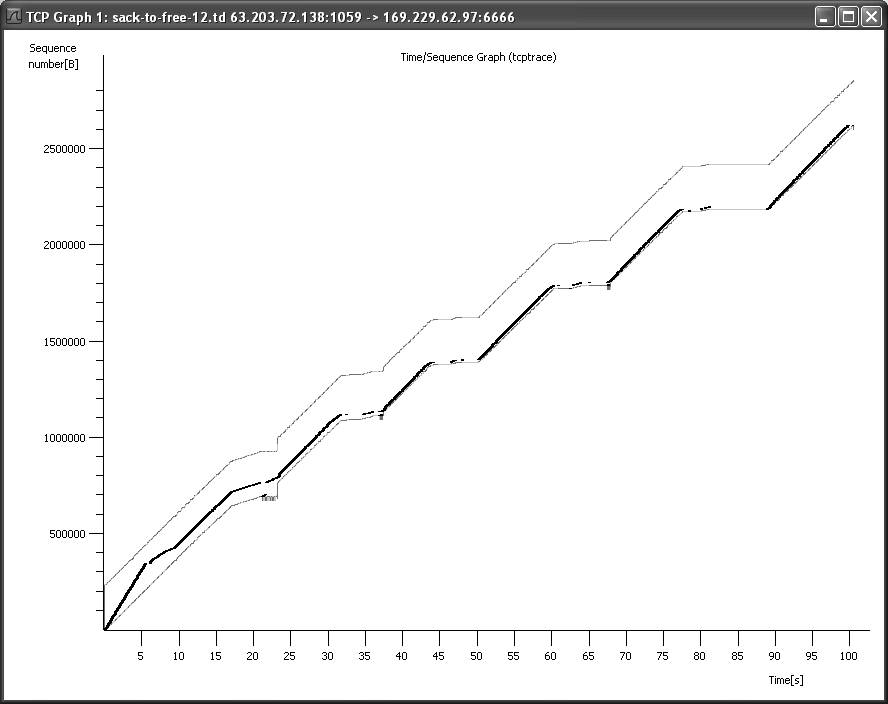
\includegraphics[width=0.7\textwidth]{imgs/16/16-4.png}
	\caption{拥塞避免算法操作。若没有 ACK延时发生,每接收一个好的ACK,就意味着发送方可继续发送1/W个新的数据包。发送窗口随时间近似呈线性增长(右,上方曲线)。当有ACK 延时,
    如每隔一个数据包生成一个 ACK,cwnd 仍近似星线性增长,只是增幅较小(右,下方曲线)}
\end{figure}

图16-4的y轴表示 TCP 序列号,每小格代表100000个序列号。x 轴是时间,以秒为单位。黑体实线由许多小的1字形线段组成,每段代表TCP 序列号范围。1形线段的最高
点表示用户数据负载大小,以字节为单位。线段的斜率为数据到达速率。斜率减小表示出现重传。在给定时间范围内的线段斜率,代表了该时间段内的平均吞吐量。从图中可以看
到,在100s时刻,发送的最大序列号为260000,表示粗略地对平均优质吞吐量的估计值为26 000B/s,这与前面对 tcptrace 输出结果的分析相一致。

图中上方曲线为接收端在对应时刻可接收数据的最大序列号(最大通知窗口)。可以看到,在起始时刻,其值约为 250000, teptrace 输出中的b->a 栏中的精确数据显示为233016。
下方曲线代表发送端在对应时刻接收到的最大 ACK 号。之前已经提到过,当 TCP 进行操作时,会增大拥塞窗口,以获取新的带宽。这和接收端的通告窗口并不冲突。这一点可以从
图中看出,随着时间推移,实线部分逐渐从下方曲线向上方曲线靠近。若始终达不到上方曲线,影响网络吞吐量的主要因素可能为发送端或者网络传输资源的限制。若黑线部分始终紧
贴下方曲线,则影响因素主要在于接收窗口限制。

Linux 2.6.10 TCP 发送端传输 2.5MB文件的 Wireshark 记录,DSL 线路速率约为300Kb/s。黑体实线代表发送序列号。上方曲线为接收端通知窗口的最高序列号(窗口右边界),下方曲线
表示发送方接收到的最大 ACK 号。图中标记的11个事件为拥塞窗口的变化情况

\subsection{慢启动行为}
在分析之前,首先观察我们之前介绍过的慢启动算法的相关操作。在Wireshark 中选择记录结果的第一个包,利用菜单中的“统计|流图”(Stafistes| Flow Graph)功能,捕绘出在
连接初始阶段包交换的过程(参见图16-5)。

\begin{figure}[!htb]
    \centering
	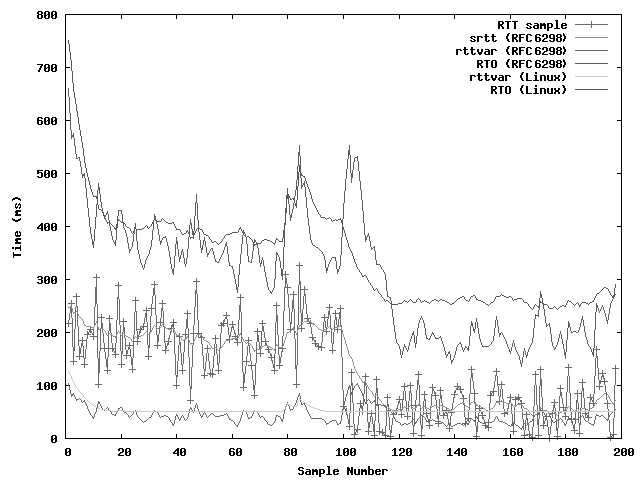
\includegraphics[width=0.7\textwidth]{imgs/14/14-3.png}
	\caption{拥塞避免算法操作。若没有 ACK延时发生,每接收一个好的ACK,就意味着发送方可继续发送1/W个新的数据包。发送窗口随时间近似呈线性增长(右,上方曲线)。当有ACK 延时,
    如每隔一个数据包生成一个 ACK,cwnd 仍近似星线性增长,只是增幅较小(右,下方曲线)}
\end{figure}

从图中可以看到初始阶段的SYN 和SYN+ACK 的交换过程。0.032s 时刻的ACK 是一次窗口更新(参见第15 章)。前两次数据包传输出现在0.126s和0.127s时刻。在0.210s时
刻返回的ACK 不是仅对一个数据包的确认。它的序列号为2801,由于 TCP ACK 的累积确认性质,它是对前两个发送的数据包的响应。这是延时ACK 的一个例子,延时ACK 通常是
每两个数据包生成一个 ACK(或如[RFC5681] 中建议的更频繁)。对接收端(FreeBSD 5.4)来说更为特殊,它需要在每个ACK 确认一个包和两个包之间切换。这表明平均来说,每三
个数据包会返回两个 ACK(假设没有出现传输错误和重传)。在第15 章中我们已经讨论过延时 ACK 和窗口更新问题了。

-个 ACK 完成对两个数据包的确认,使得滑动窗口可以向前滑动两个包,因此可以继续发送两个新的数据包。由于连接处于初始慢启动阶段,发送端每接收一个好的 ACK,
拥塞窗口相应加1(Linux TCP 管理的拥塞窗口以包为单位)。在上述情况下,cwnd 从2增至3。因此可以继续传输三个数据包,分别在0.2158、0.216s 和0.217s时刻发送。

0.264s到达的ACK 是对单个包的确认,表明接收方期望下次接收序列号为4201 的数据包。然而,4201 号以及之后的5601 号数据包已被发送,但仍未到达。因此,0.264S时刻的
ACK使得cwnd 由3变力4,但由于两个包仍处于传送状态,只能允许继续发送两个数据包(该ACK 使得滑动窗口前行,另外,接收到这个好的ACK 允许
cwnd 加1)。这两个包的发送时间为 0.268s和 0.268s(在同一个 1/1000秒内)。

以上是发送端执行慢启动情况下接收端延时返回 ACK 的典型例子。这个过程持续(每接收一个 ACK 发送两三个新数据包)直到5.6S。下面我们进一步讨论此时发生的情况。

\subsection{发送暂停和本地拥塞(事件1)}

如图16-4所示,在5.512s 时刻发送一个数据段后,直到6.162s 时刻才开始再次发送,这中间出现了一个暂停。利用Wireshark 的图像放大功能可以得到图16-6。

可以看到,在发送暂停阶段没有新数据的传输,也没有重传,但暂停结束后却出现了传输速率的下降,这是为什么呢?我们再次通过传输流记录功能一探究竟(参见图16-7)。

暂停前最后一次传输的数据段开启了 PSH标志,表明发送缓存已经清空,所以在S.SS9s时刻TCP发送端已经终止发送。导致发送终止的原因可能有多种,如发送方系统忙于
处理其他任务,无暇顾及数据传输。

我们可以看到这次暂停并不意味着重传恢复阶段的开始,但暂停结束后线段的斜率有所下降,表明发送速率在减小。下面将仔细观察并探讨这种行为产生的原因。

暂停前最后发送数据的序列号为343001+1400-1=344400,该序列号之前没有发送过,所以不是重传数据。在5.486s时刻(已标记出)发送完数据段后,网络中己发出但未收
到 ACK 的数据量达到最大值:341 601 +1400- 205 801 = 137 200字节(98个包),即 cwnd值为98个包。5.556s时刻到达的 ACK 表明又有两个包被成功接收。暂停前最后又发送了一
个数据包,序列号为344400,这样一共有97个包还来成功接收。

\begin{figure}[!htb]
    \centering
	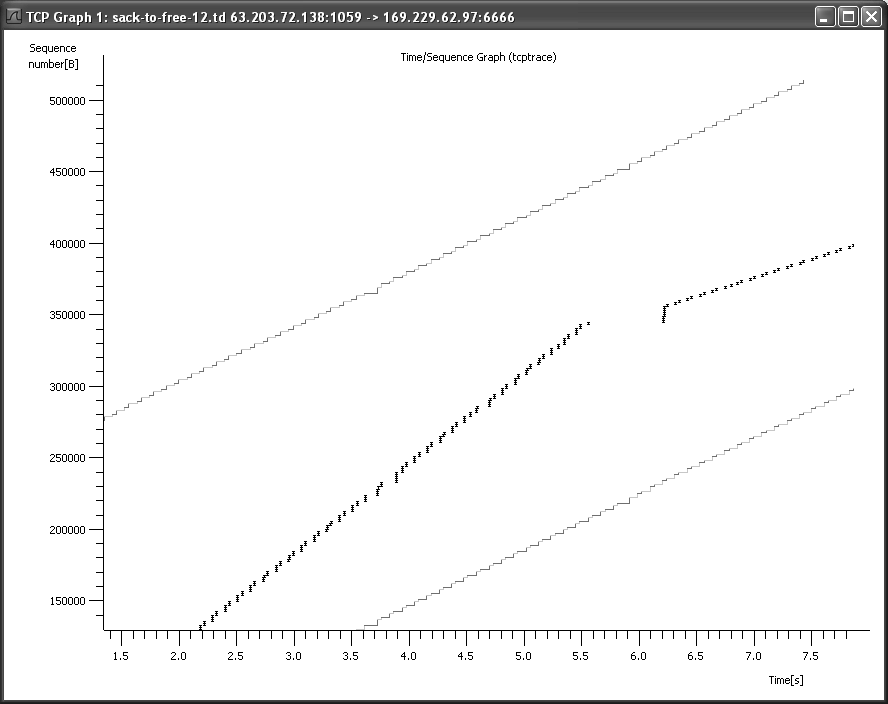
\includegraphics[width=0.7\textwidth]{imgs/16/16-6.png}
	\caption{在慢启动阶段后,连接暂停持续了约512ms,接着在5.512s时刻恢复发送}
\end{figure}


在发送暂停阶段,共有11个ACK 到达(之前提过,每个 ACK确认一个或两个数据段)。最后一个 ACK 表明序列号为233800的数据段已成功传输,同时仍有110600字节
(79个包)的数据没有收到确认。此时,发送方开始继续发送,它可以发送的数据包个数为98-79=19个,但从图中看到,它只发送了8个。至6.128s,它发送的数据段的最终序列
号为354201+1400-1=355600。

从传输流记录图中并不能很清楚地看到 TCP 当时的状况。我们预料应该会发送19个包,但结果只发送了8个。原因可能在于,下层产生的大量数据包堵塞了本地(下层)队列,
使得后续包无法传送。为明确是否由下层原因导致上述问题,由于数据包经过 PppO网络接口传输,所以在 Linux 中使用如下命令:
\begin{figure}[!htb]
    \centering
	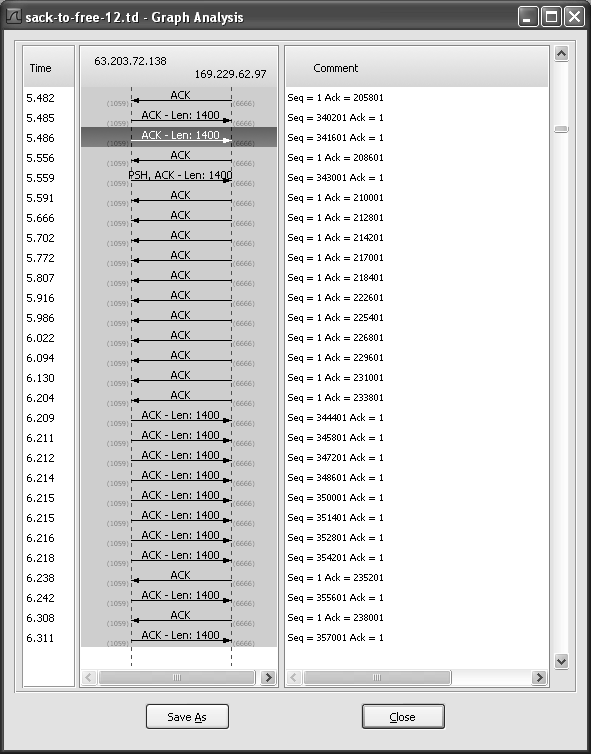
\includegraphics[width=0.7\textwidth]{imgs/16/16-7.png}
	\caption{在5.5S9s 时刻发送方暂停发送。6.209s时刻重新开始发送,由于本地拥塞,可发送包个数被限制为8个。有些TCP 版本就是利用限制发送速率的方法来避免发送端队列拥塞}
\end{figure}

\begin{verbatim}
    Linuxs te -s -d adise show dev pppO gdisc pfifo_fast 0: bands
3 prionap
1222120011111111
Sent 122569547 bytes 348574 pkts (dropped 2,
overlimits
0 requeues 0)
\end{verbatim}

上述命令中的tc 是Linux 中用于管理包调度和流量控制子系统的指令[LARTC]。-s 和-d选项提供具体的记录细节。指令 qdise show dev pppO 为显示设备pppO的排队规则,即管理
和调度包发送的方法。注意到这里出现了两个丢包,这不是在网络传输过程中的丢包,而是出现在发送端 TCP 下层的丢包。由于丢包发生于 TCP 层以下,但又是在包的操作处理层以
上,所以传输流记录中并不记录这些包,这也是我们只看到8个包传输的原因。在发送端系统产生的丢包有时称为本地拥塞,产生原因在于,TCP产生数据包的速度大于下层队列的发
送速度。

\begin{tcolorbox}
    Linux流量控制子系统以及一些路由器和操作系统支持的优先级策略或 QoS特性(如 Microsoft 的qWave API[WQOS]),可能使用不同的排队规则,按照数据
    包的特性(如IP DSCP 值或 TCP端口号)会有不同的调度方法。对某些数据包(如多媒体数据包,TCP纯ACK 包等)采用优先级策略,可以提升交互式应用的用户
    体验。一般来说,互联网并不支持优先级策略,但许多局域网和有些企业 IP 网络中会采用这种策略。
\end{tcolorbox}

本地拥塞是 Linux TCP 实行拥塞窗口缩减(Congestion Window Reducing, CWR)策略[SK02]的原因之一。首先,将 ssthresh 值设置为cwnd/2,并将 cwnd设力min (cwnd.,在
外数据值+1)。在CWR 阶段,发送方每接收两个 ACK 就将cwnd 减1,直到cwnd达到新的ssthresh 值或者由于其他原因结束CWR(如出现丢包)。这本质上和前面提到的速率减半
(rate-halving) 算法一致。若 TCP 发送端接收到 TCP 头部中的 ECN-Echo 也会进入CWR状态(参见16.1.1节)。

了解了这些之后,我们就可以理解前面情况的产生原因了。当 TCP 结束暂停后,它只能继续发送8个包。由于本地拥塞,无法传输额外的包,TCP进入CWR状态。ssthresh 立
即减为98/2 =49个包,cwnd 也变为79+8=87个包。每接收两个 ACK,cwnd 就会减1,这样就导致发送速率减慢,直到8.364s时刻cwnd 值变为66个包。

发送速率的减小也可以从图16-6中观察出来,在5.5s 时刻前,线段的斜率显示数据传输速率约为 500Kb/S。这个值大于传输方向上的最大速率,必然会使得链路中的一个或多
个队列出现拥堵,导致 RTT增大。我们可通过“统计ITCP 流图IRTT 图”(Statistics | TCPStream Graph | Round Trip Time Graph) 进行观察(参见图16-8)。

\begin{figure}[!htb]
    \centering
	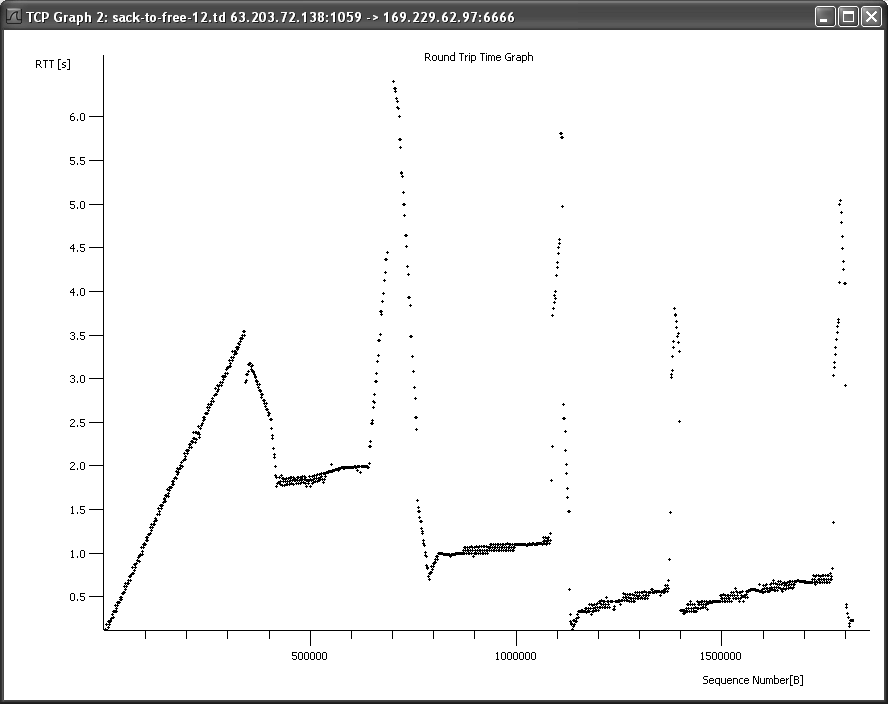
\includegraphics[width=0.7\textwidth]{imgs/16/16-8.png}
	\caption{发送端对 RTT 的估计值曲线。RTT增长阶段(图中稠密的增长值群组)对应于由过大的发送速率导致路由器缓存溢出的情况,RTT 降低阶段则表示发送端减慢发送速率,等待队列逐渐减小}
\end{figure}

如图16-8所示,y轴代表 RTT估计值,以秒为单位。x 轴表示序列号。可以看到,在序列号约为340000处,RTT 开始减小。这和之前提到的发送暂停前最后发送的序列号相一致
(344400)。RTT 的减小意味着发送方减慢发送速率,使得网络传输负载减轻(即数据发出速率大于新数据到达速率)。这样路由器队列逐渐为空,等待时间减小,RTT也相应減小。
TCP 处于CWR状态,发送速率会持续减小。最终,RTT 会减至绝对最小值约17ms。通常,TCP 会避免这种情况的发生,因为它需要保持传输通道处于“满”的状态,以此确保
充分利用可用的网络资源。

\subsection{延伸 ACK 和本地拥塞恢复}
在8.3645时刻,随着进入CWR状态 cwnd 逐渐减小,使得 TCP 传输速率更快地减小。从8.362s时刻的 ACK 可以得到在外数据值,cwnd 与这部分在外数据量的关系导致了发送速
率的快速降低(图16-9中标记部分)。

8.362s 时刻的ACK 号为317801,而前一个ACK 是313601,所以这个ACK 确认的数据为 317801 -313 601=4200字节(3个包)。这通常称为延伸 ACK(stretch ACK),即一个
ACK 确认两个最大段以上长度的数据。其形成原因有多种,最简单的就是ACK 丢失。通常很难判断延伸ACK产生的确切原因,但这并不重要。在这个例子里,我们假设先前的ACK
丢失。这个延伸 ACK 使得 cwnd 从 68减为66。

\begin{figure}[!htb]
    \centering
	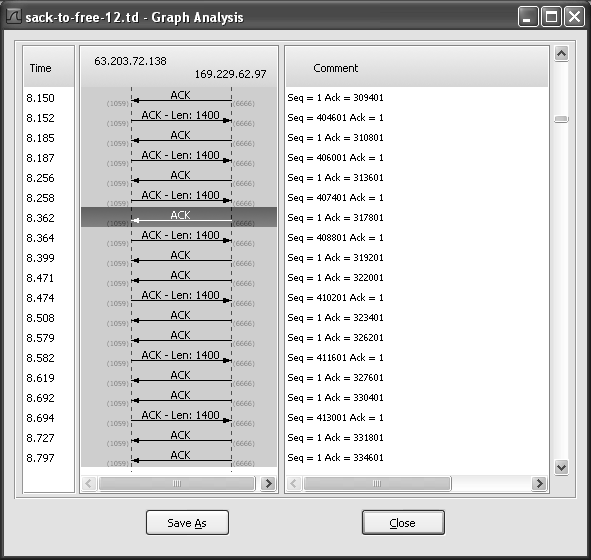
\includegraphics[width=0.7\textwidth]{imgs/16/16-9.png}
	\caption{一个“延伸 ACK”确认了三个数据包长度的数据。这种 ACK 可能使得发送端突发操作,当其他 ACK 在传输中丢失时,可能会出现延伸ACK}
\end{figure}

Linux 的TCP实现在每次接收 ACK 时,总是试图调整已发送但未经确认数据(记为在外数据,outstanding data)的估计值。(当它发送数据段后,也会根据之前提到的拥塞窗口校
验算法去修改拥塞窗口,但这里并不生效。)在CWR 阶段,如果在外数据包由于某种原因减少,如这里的接收延伸 ACK 后,cwnd 调整为在外数据估计值加1。需要注意的是,CWR通
常只会在接收到每一对ACK 后将 cwnd的值減1,因此这是额外的操作。通常情况下每接收一个 ACK, cwnd 会减小1 或0,然后 cwnd 被设置为 min(在外数据值+1,[也可能减少的〕
cwnd)。CWR 阶段一直持续到 cwnd达到 ssthresh 或其他事件的发生,如丟包或重传。

在收到延伸ACK 前的8.258s 时刻,在外数据估计值为407 401 +1400 -313601=95 200字节(68个包)。接收延伸 ACK 后,在外数据包为65 个,cwnd 调整为66。
在CWR 阶段,在外数据估计值和cwnd 紧密相关。在这里出现了ACK 延时的情况,导致每两个 ACK 到达cwnd 值减2,但只能发送一个新数据包。原因如下:假设在 ACK 到达前,
cwnd 值co,在外数据估计值f6=co。当第一个 ACK 到达(对一个包的确认),尤=f6-1,cwnd 更新 ci =min (co - 1,f+1)=co-1。当第二个 ACK 到达(由于延时 ACK,因此为对
两个包的确认),½=f-2=co-3, cwnd设 cz = min (Ci,5+1)=min (Co-1,c0 -2)=Co -2。至此拥塞窗口减2,但已有3个包被确认,因此在接收第二个 ACK 后,只可继续发送一个包。
\begin{figure}[!htb]
    \centering
	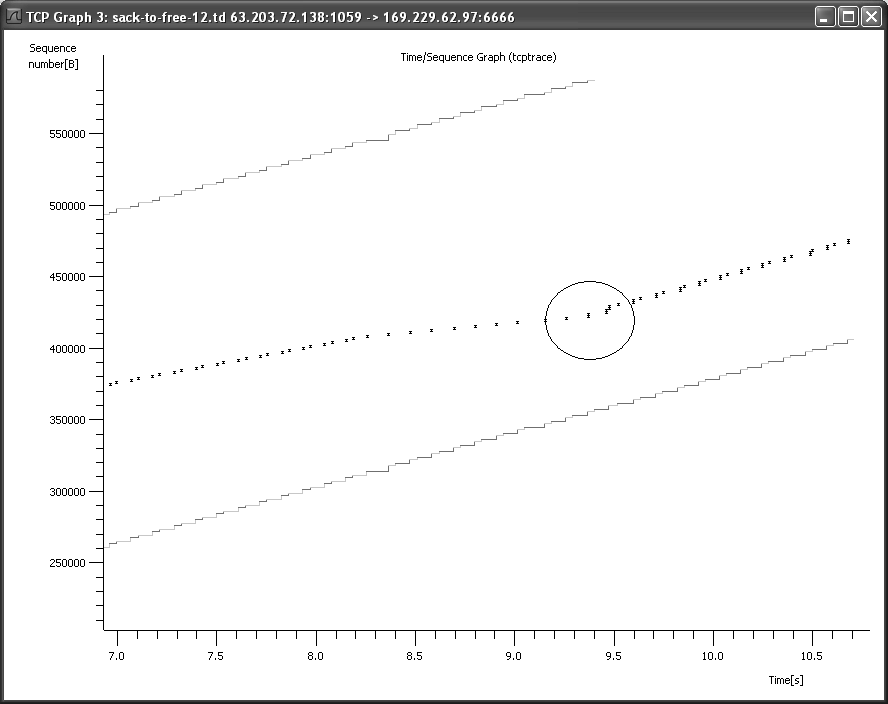
\includegraphics[width=0.7\textwidth]{imgs/16/16-10.png}
	\caption{在9.37s时刻,cwnd达到 ssthresh 为49,发送端结束CWR阶段。TCP 返回正常操作模式,继续执行拥塞避免(参见图16-10和图16-11)}
\end{figure}

在图16-10中,用圆圈标记出的数据包表明发送端结束CWR,继续执行拥塞避免算法。图16-11更为详细地显示了这一行为。

发送端继续执行拥塞避免,逐渐达到相对稳定的吞吐量。然而,在17.232s 时刻,开始形成严重的拥塞,致使RTT 大幅增长。在图16-8 中可以看到,在序列号 720000处,RTT约
增至6.5s—是稳定阶段(2s)的三倍多。这是大规模拥塞的常见现象。最终,严重的网络拥塞导致了丢包,TCP发送端开始了首次重传。
\begin{figure}[!htb]
    \centering
	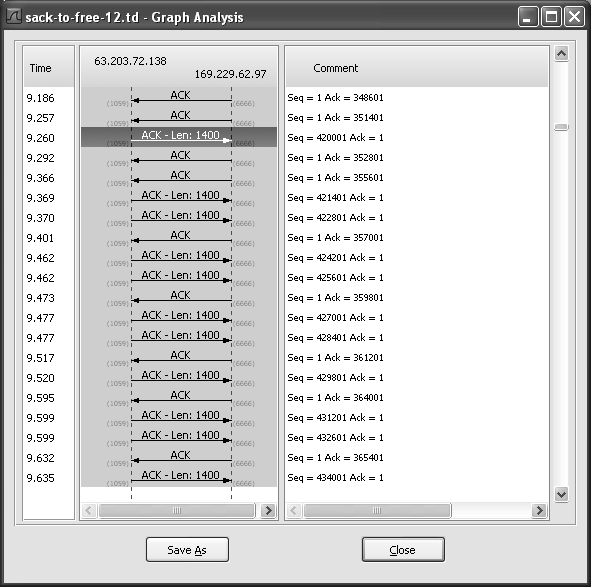
\includegraphics[width=0.7\textwidth]{imgs/16/16-11.png}
	\caption{TCP 完成了恢复阶段并返回正常(拥塞避免)状态。每接收一个 ACK 就发送一个或两个新的数据包}
\end{figure}
至9.369s时刻,发送端恢复正常模式,继续执行每接收一个 ACK 发送一个或两个新数据包操作

\subsection{快速重传和 SACK 恢复(事件2)}

由于RTT 大幅增长,在21.209s时刻出现了首次重传。从图16-12 可以清楚地看到,首次重传(图中圈出部分)数据包的起始序列号为690201,对应接收到的最高 ACK 号(也是
690201)。这次重传是由于接收到带有SACK 块为[698601,700001]的重复 ACK,这里的数值区间是接收端成功接收的序列号区间,表明这是对单个数据包的确认。
\begin{figure}[!htb]
    \centering
	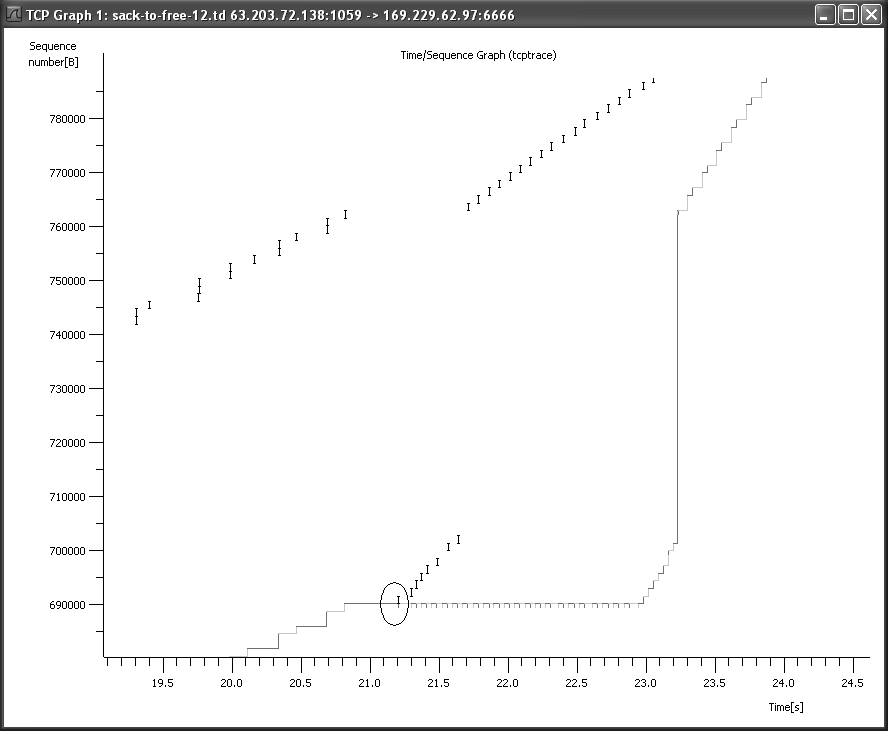
\includegraphics[width=1\textwidth]{imgs/16/16-12.png}
	\caption{首次重传(已圈出)发生在21.209s时刻。SACK 块用于告知发送方发送哪些数据包。在21.0~22.0s时间内,共出现了8次重传}
\end{figure}

至21.209s时刻首次重传发生为止,已发送数据的最大序列号为761601 + 1400 -1=763000,cwnd 值 52。重传发生后,ssthresh 值从49 减为26,TCP 进入恢复阶段,一直持续
至接收到序列号为 763000(或更高)的累积 ACK 为止。另外,cwnd 也减为(在外数据值+1)。由于有些数据很可能已丢失,因此并不能直接确定在外数据值,需要利用下式:
\begin{equation}
    flight size(在外数据值)=packets_outstanding + packets_retransmitted - packets_removed
\end{equation}
等式右边的第一项表示经首次发送(非重传)但仍未收到 ACK 的数据;第二项为重传但仍未经ACK 确认的数据;最后一项则表示那些网络中已经不存在,但还没有收到ACK的
数据。由于 TCP 无法确认获知最后一项 \verb|packets_removed| 值,因此必须通过估算的方法。它包括已被接收(失序)的数据加上在传输中丢失的部分。利用SACK 可以知道前半部分的值,
但丢包个数仍需要估算。

\verb|packets_outstanding| 的计算值(763 001 - 690 201)/ 1400 = 72800/1400 = 52。根据SACK 块的序列号区间,可以推算出已被接收缓存的包个数为(700 001 - 698601)/1400=
1400/1400 =1。利用FACK(这里默认启用),经 SACK 推算出的级存之间的空缺被认为是丢包。这里估算共有 698 601 -690201 -8400(6个包)丢失。因此,fight size 的值为52+1-
(1+6)-46,相应地,cwnd值设为47。与CWR 相似,在恢复阶段,每接收两个包的 ACK,cwnd减1。首次重传后,又发生了7次重传。接着在21.2~21.7s时间内,又开始了新数据
的发送,相应的每个 ACK 都包含了 SACK 信息(參见图16-13)。

图16-13 去换了 Wireshark 中其他不相关信息,可以清楚地看到每个 ACK 包含的SACK信息。观察 SACK 的序列号区间(SLE 和 SRE),有两个常见值:[698601,700001]和
[702801,763001]。前者表示只缓存了一个数据包(序列号范围为 698601 ~700001),后者则增加至 43个包(序列号范围为 702801 ~763001)。通常CWR阶段的速率波半算法每接
收两个包,cwnd 至少减1。这里每个 ACK 是对一个包的确认,flight size 相应减1,因此可以发送一个新的数据包。注意这里和CWR状态的区别,CWR 情况下,每个 ACK 提供对两
个包的确认,而这里一个 ACK只确认一个包,因此不论是否为重传包,每接收一个 ACK,cvnd减1。在整个恢复期间,cwnd 从47减为20。

Wireshark 显示,大多数包含SACK 的ACK 是序列号为 690201 的重复ACK(其中44个)。有5个好 ACK 为包含 SACK 块[702801,763001]和 [698601,700001]的非重复ACK。还有
两个 ACK 只包含了1702801,763001]SACK块。这些ACK 并不能使发送端结束恢复状态,因为ACK 号低于之前提到的763000(恢复点)。它们属于我们在前面讨论过的局部 ACK。

23.301s 时刻接收了序列号为 765801(大于前面提到的763000)的好ACK,表明已经达到恢复点,此时的cwnd 为20,ssthresh 值为26,说明TCP正处于慢启动状态。又经历
几轮传输后,到23.659s时刻,cwnd达到27,TCP恢复正常操作,继续执行拥塞避免算法。至此首个快速重传恢复阶段完成。

\subsection{其他本地拥塞和快速重传事件}
下面再次发生了本地拥塞、快速重传和其他两个本地拥塞相关事件。它们和之前的相关内容有相似的地方,这里只是进行简要概括。
\begin{figure}[!htb]
    \centering
	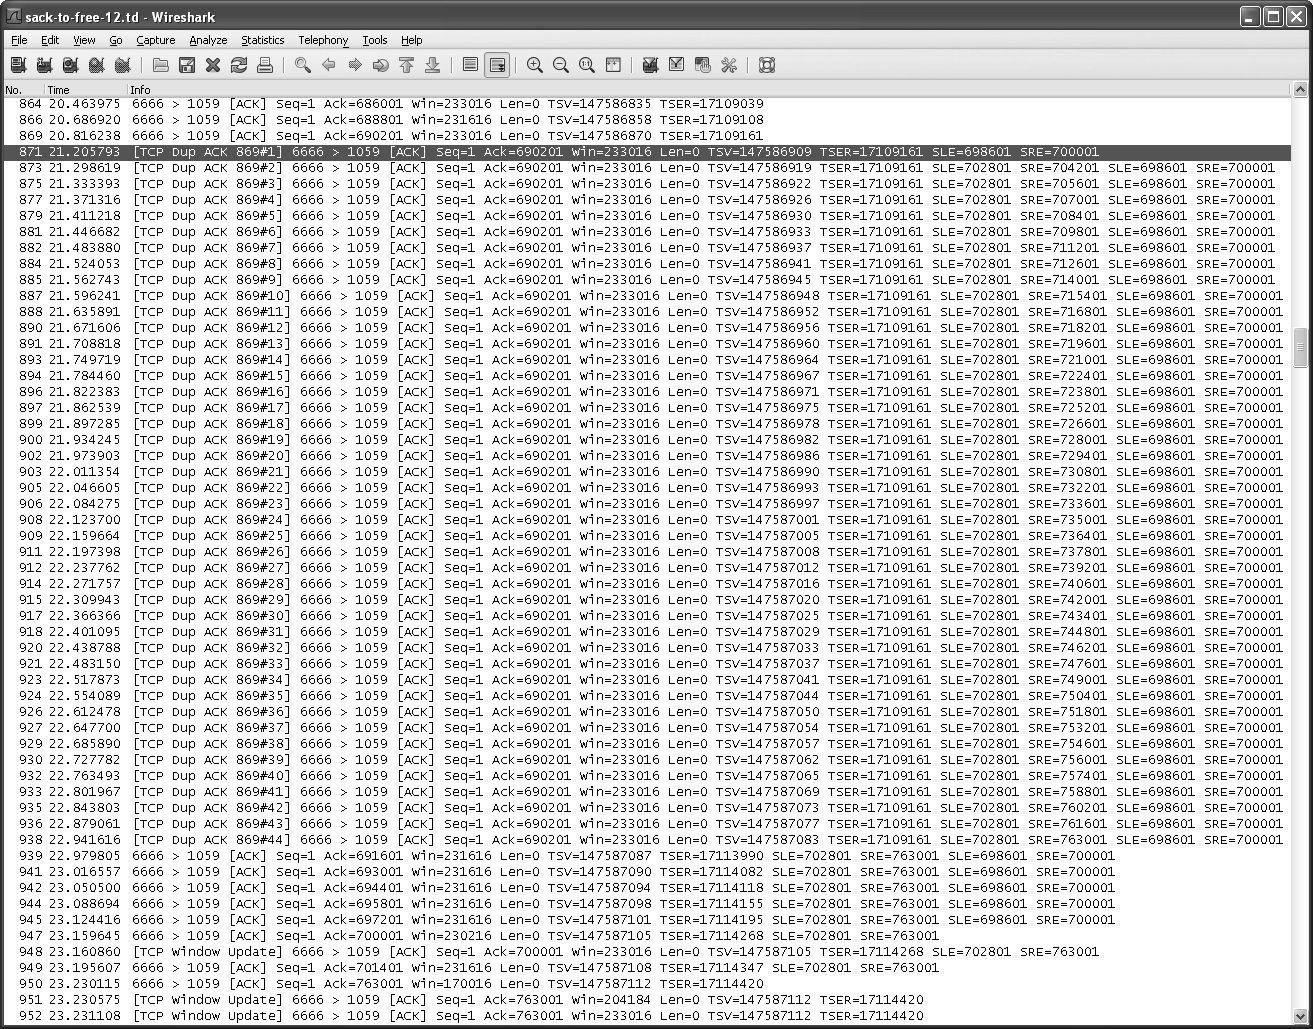
\includegraphics[width=1\textwidth]{imgs/16/16-13.png}
	\caption{首次重传(已圈出)发生在21.209s时刻}
\end{figure}
\subsubsection{再次 CWR(事件3)}
在30.745s时刻,由于本地拥塞再次出现了CWR事件。此时在外数据值为1 090601+1400-1 051 401 =4060029 个包),cwnd 为31。按理可再发送两个包,但由于出现本地拥塞,
导致实际并未发送。在这种情况下,cwnd 被设置为在外数据值+1 = 30, ssthresh 减为15。在34.759s时刻,在RTT 再次出现大幅增长后,cwnd 降为 ssthresh 时,TCP退出CWR状态。

\subsubsection{二次快速重传(事件4)}
在36.914s时刻,cwnd =16,再次出现快速重传。利用 Wireshark 的基本显示功能,可以清楚地看到重传(参见图16-14)。
\begin{figure}[!htb]
    \centering
	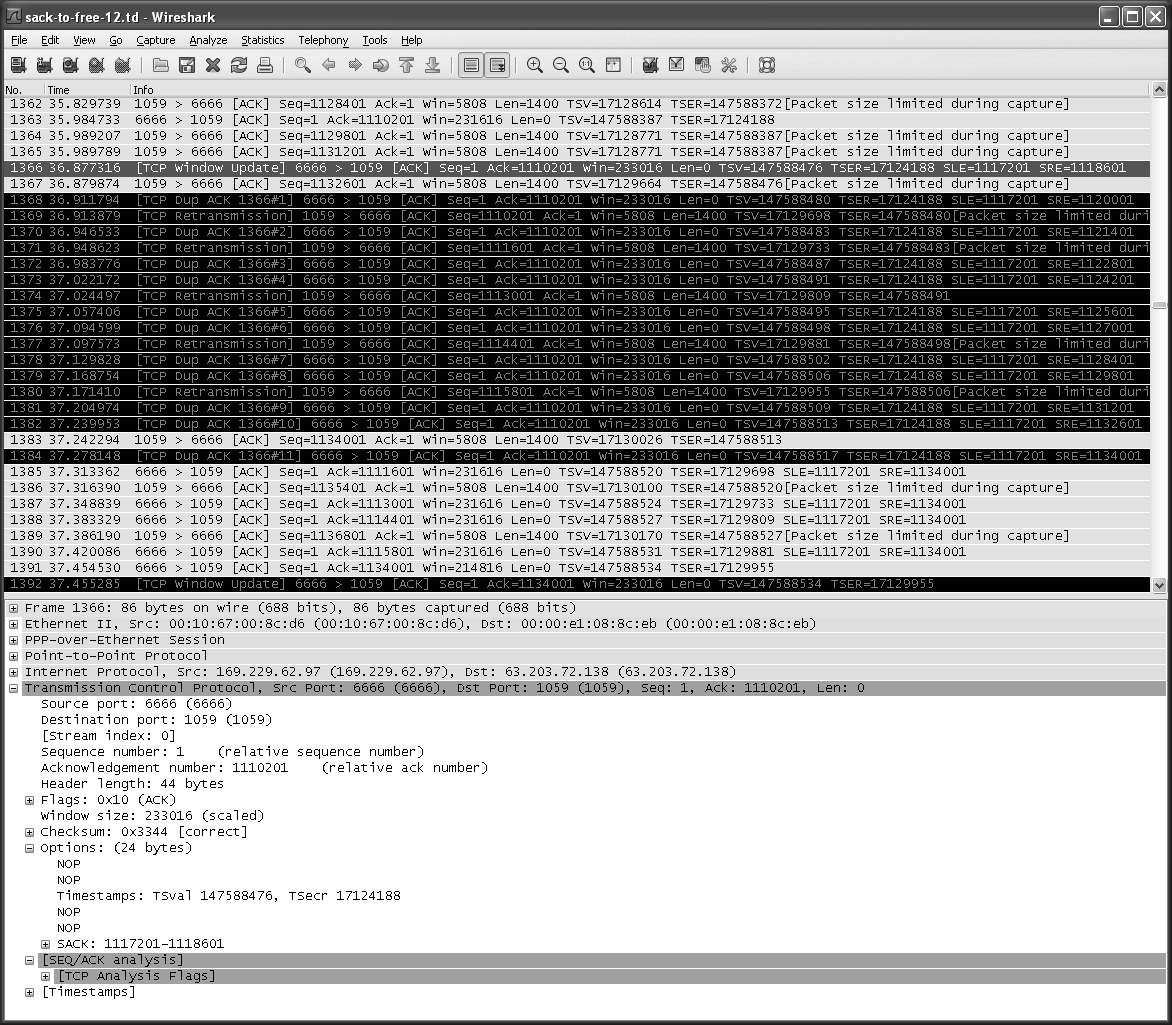
\includegraphics[width=1\textwidth]{imgs/16/16-14.png}
	\caption{linux}
\end{figure}
在36.878s时刻,接收了一个带SACK块[1117201,1118601]的ACK (1366号包,ACK号为1110201)。这使得Linux TCP 进入了失序状态,到达一个 ACK 就能触发一个新
效据包的传输(和限制传输相似),1367号包就是经该ACK 触发发送的。

一旦接收到一个重复ACK 或一个带SACK 信息的ACK, Linux TCP 发送端会进入失序(Disorder)状态。在此状态下,数据包的到达会触发新数据的传输。之后再次接收重复(或带SACK 信息的)ACK,就会进人恢复(Recovery)状态,并开始重传

36.912s时刻接收了包含SACK块[1117201,1120001]的重复ACK (1368号包),因此TCP 进入恢复阶段,并在36.914s 时刻触发快速重传(1369号包)。至此已发送数据的最大序列
号为1132601+1400 1 113400。随者37435日 时刻序列号为 1134001的ACK(1331号包)到达,恢复阶段结束。注意到紧随这个 ACK 的是一次窗口更新。对于批量数据传输来说,接
收窗口相对于网络带宽延迟积较大,因此这样的窗口更新通常不是很重要。但在交互式传输、接收窗口较小或者很少从网络中读数据的传输中,这些更新就相当重要(第15 章已经
提到)。当36.914s 时刻的第一次快速重传开始,ssthresh 从 16 减为8。到37.455s 时刻恢复阶段完成,cwnd =4, ssthresh =8。由于 cwnd 小于 ssthresh,发送端进入慢启动状态。

\subsubsection{再次 CWR(事件5和事件6)}
随着43.356s时刻序列号为1359401的ACK 的到达,由于本地拥塞致使后续数据包无法发送,TCP 再次进入CWR状态。这使得 ssthresh 减为8,cwnd 变为15。在CWR状态的
再次传输失败,致使 ssthresh 变为12。最终结束 CWR 时,cwnd=7, ssthresh =8。

另一次的本地拥塞发生在 59.6525 时刻,此时的 cwnd = 19, ssthresh = 10,导致 TCP 再次进入CWR状态。这次出现了超时,致使 TCP 由CWR状态进入丢失(Loss)状态。这是
我们需要讨论的新的事件类型。

\subsection{超时、重传和撤销 cwnd 修改}
TCP 设置了超时计时器,用于快速重传中出现丢包的情况。至此我们还没有看到重传超时的发生,这从一定角度说是好事,因为一旦超时发生,就意味着网络中出现了严重的拥
塞,性能极差。在下面的传输过程中,如图 16-15所示,我们将看到重传计时器超时后TCP的处理操作。

发送端经历了首次超时,其 RTO=1.57S。在这里,发送端认为这是一次伪超时,并撤销了对拥塞控制变量的变更

\subsubsection{首次超时(事件7)}
62.486s时刻出现了一次重传(2157号包),序列号为1773801(图16-15中标记部分)、在此之前,并没有重复 ACK 或SACK 信息。
\begin{figure}[!htb]
    \centering
	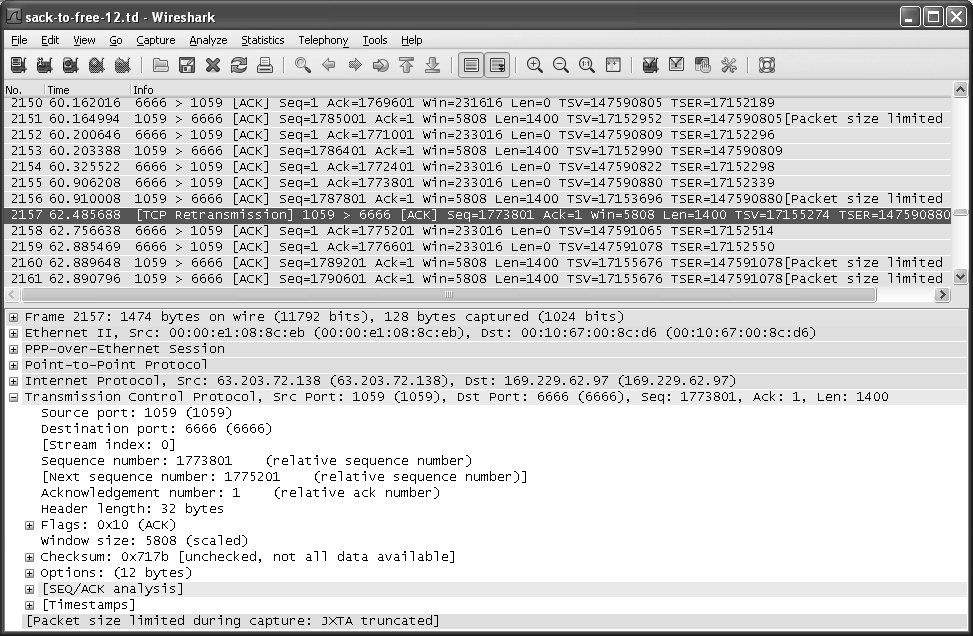
\includegraphics[width=1\textwidth]{imgs/16/16-15.png}
	\caption{linux}
\end{figure}
如图 16-15所示,在62.486s时刻,至上个 ACK 到达已过了1.58s,但根据图16-8,此时的 RTT估计值只有800ms。因此,我们认为发生了重传超时。TCP 进入丢失(Loss)状态,
cwnd 减小为1,ssthresh设为5,进人慢启动状态。超时也使得之前保存的SACK 信息被丢弃。然而接收端仍会返回SACK 信息,因此对新接收的 SACK 可以继续使用。

\begin{tcolorbox}
    当经历超时后,TCP 应当 “忘记”之前的SACK 信息,原因在于接收端可能会改变它之前发出的SACK信息。根据[RFC2018],当接收端需要调整其缓存
    时,可能将之前存储的失序数据删除。尽管并不常见,但这种行为是允许的。当接收端需要整理缓存时,只有第一个SACK 信息中最近接收到的数据块不会删除。
    其他的 SACK 信息都不再可信。
\end{tcolorbox}

然而有趣的是,这里的拥塞操作都撤销了。之前已经提过,当TCP认为重传超时出错会执行 Eifel 响应算法。在此处可以凭借时间戳的证据来判定出错。62.752s时刻接收的序列
号为1775201的ACK(2158号包)携带了一个 TSOPT(时间截选项),其TSV(时间戳值)为17152514,而重传包的 TSV 为17155274。由于ACK 的 TSER(时间截回显重试)字段包
含了重传的数据段,并且早于该重传包,因此认为此处的重传是无用的,接收方在重传前已经接收到了该数据段。所以重传超时也是无效的。

由于超时出错,TCP 触发了 Eifel 响应算法,恢复了 cwnd 和 ssthresh 的值,并转为正常状态,继续执行拥塞避免算法。

\subsubsection{快速重传(事件8)}
在67.510s时刻,接收了一个序列号 1789201的重复 ACK(2179号包),包含 SACK块[1792001,1793401],因此TCP 再次进入失序(Disorder)状态。至此已发送数据的最
大序列号为1806000。再次到来的 SACK 信息使得 TCP 进入恢复(Recovery)状态,并在67.550s 时刻开始了序列号为1789201 的又一次快速重传(2182号包)。这使得 ssthresh 减至
5,cwnd 也相应开始减小。随着 67.916s 时刻序列号为1806001的ACK(2197号包)到达,恢复阶段结束。

\subsubsection{再次 CWR(事件9)}
在77.121s 时刻,又一次出现了本地拥塞事件,此时的cwnd = 18。这使得 ssthresh 被置为9并再次进入CWR状态。然而,由于出现超时,这次CWR 中cwnd 的减值过程被中断,
cwnd 只减小了1,最终值为8。

\subsubsection{再次超时(事件10)}
再次超时又引发了新一轮的重传,在78.515s时刻又发送了序列号为2175601 的包(图中未标记)。cwnd 更新为1,ssthresh 仍9,重传数据段的 TSOPT TSV 值17171306。
80.093s 时刻到达的序列号2179801 的ACK(2641号包)的 TSOPT TSER 值17169948,和事件7的超时一样,拥塞操作也被撤销了。此时 flight size 估计值为2 184001 + 1400 -
2179 801 = 5600字节(4个包),由于拥塞操作撤销,因此cwnd 仍为8,这样将允许再发送4个新数据包。但这样的突发操作可能会造成丢包,所以应避免发送。

为防止这种突发行为,Linux TCP 实现了拥塞窗口调整(congestion window moderation)机制。它将单个ACK 能触发的新数据包发送个数限制为最大突发值(maxburst),这里取值
为3。因此,cwnd被设置为(在外数据值+最大突出值)=4+3=7。拥塞窗口调整机制和TCP 中的相关方法一致,并经网络仿真工具 NS-2验证。NS-2 在开发和探讨新的TCP 算法
研究中被广泛使用。

\subsubsection{超时和最后一次恢复(事件11)}
如图 16-16所示,在88.929s时刻出现了重传计时器超时,引发了序列号为2185401数据包的重传。
\begin{figure}[!htb]
    \centering
	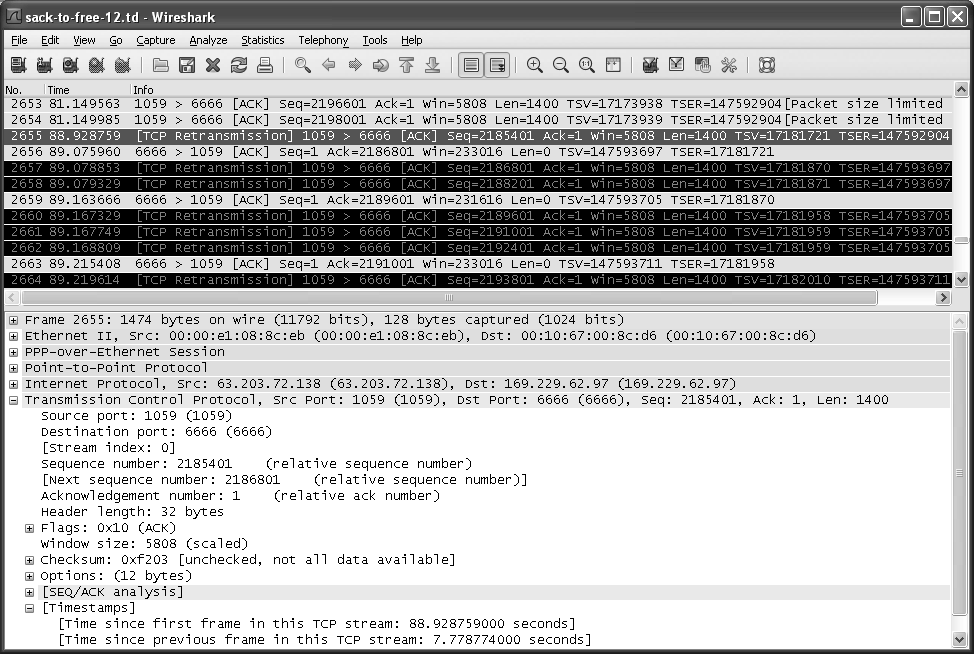
\includegraphics[width=0.7\textwidth]{imgs/16/16-16.png}
	\caption{linux}
\end{figure}
这次超时使得发送端进入慢启动状态,ssthresh=5。这次 TCP 不能撤销超时,因此cwnd被置为1,继续执行慢启动。从下面的传输流记录图可以更清楚地观察(参见图16-17)。
\begin{figure}[!htb]
    \centering
	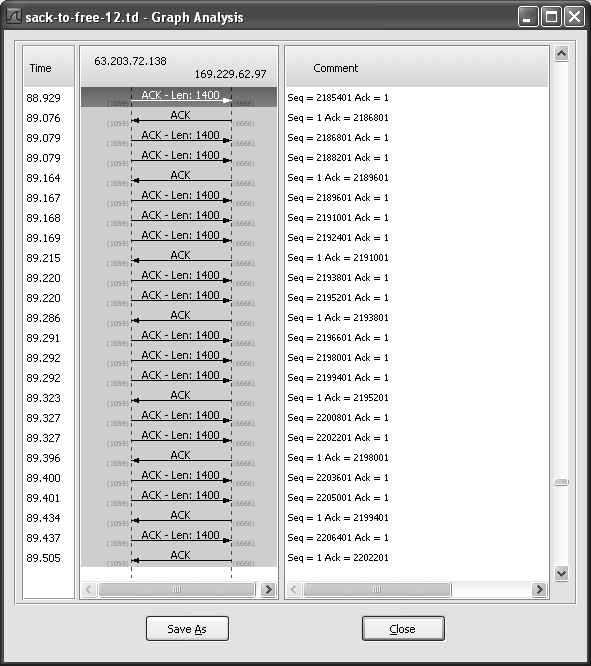
\includegraphics[width=0.7\textwidth]{imgs/16/16-17.png}
	\caption{linux}
\end{figure}
序列号为2185401的重传已在图中标出。在重传后,与连接建立初始一样,开始了慢启动操作。根据每个到达 ACK 确认的数据包个数,继续发送两个或三个新数据包。直到
89.4345,cwnd 达到 ssthresh 的值(5),TCP 继续执行拥塞避免。

\subsection{连接结束}
最后一次包交换传输中,首先发送方在99.757s时刻发送了一个FIN 包。接着接收方返回了13个ACK和一个FIN 包。在100.476s 时刻发送了最后一个包(即最后的ACK)。该交
换过程参见图 16-18。
\begin{figure}[!htb]
    \centering
	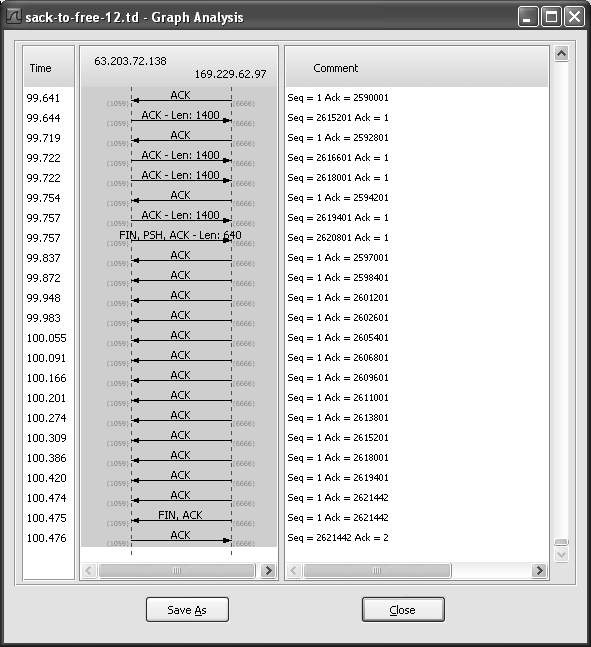
\includegraphics[width=0.7\textwidth]{imgs/16/16-18.png}
	\caption{在连接关闭过程中,接收端返回了 13个纯 ACK 来确认发送端发送的所有数据都已成功接收。最后的FIN-ACK 传输关闭了接收端至发送端的连接。注意 FIN 报文段包含了有效的ACK号}
\end{figure}

传输的最大序列号为 2620801+640-1=2621440,等于总共传输数据大小2.5MB。在99.757s 时刻,在外数据量为(2619 401+1400-2 594 201)/1400+1 =20个包。到达的13
个ACK(其中7个是对两个包的确认)完成了全部(2*7)+(13-7)=20个包的确认。注意到100.472s 时刻达到的 ACK 确认的两个数据包长度分别为1400和 640,分别对应2 621442 -
2619 401 =1400+640。

这个扩展示例涉及了我们之前讨论过的大部分算法,包括基本TCP 算法(慢启动、据塞避免)以及选择确认、速率减半,包括一些比较新的方法如伪 RTO 检测等。下面我们将
讨论一些算法的改进,以及那些不太普遍但更具理论性或者更新的方法。Linux TOP 协议栈实现了很多这样的方法,但不是默认启用的。通常只要利用 sysetl程序稍加修改就能使用。
Windows 的一些较新版本(Windows Vista 及以后版本)也都实现了这些功能的改进。

\section{共享拥塞状态信息}
前面的讨论和举例都是针对单一的TCP 连接的拥塞处理操作。然而,相同的主机之间随后可能建立新的连接,这些新连接也需要重新进行拥塞处理,建立自己的 ssthresh 和 cwnd
值。在许多情况下,新连接可能会用到相同主机之间的其他连接的信息,包括已关闭的连接或者正处于活动状态的其他连接。这就是相同主机间多个连接共享拥塞状态信息。之前的一
篇名为“TCP控制块相互依赖性”的文章[RFC2140]描述了相关内容,其中注意区分了暂时共享(temporal sharing,新连接与已关闭连接间的信息共享)和总体共享(ensemble sharing,
新连接与其他活动连接间的信息共享)。

为将上述思想形成除 TCP 外的新的应用协议,[RFC3124]提出了拥塞管理(CongestionManager)机制。该机制使得本地操作系统可实现相关协议来了解链路状态信息,如丢包率、
拥塞估计、RTT等。

Linux 在包含路由信息的子系统中实现了上述思想,即第15 章已经提到的目的度量。这些度量默认开启(在前面的扩展示例中,我们通过设置 sysctl 变量 \verb|net.ipv4.top_no_metrics_save|
为1禁用了该项功能)。当一个 TCP 连接关闭前,需要保存以下信息:RTT 测量值(包括 srtt 和 rttvar)、重排估计值以及拥塞控制变量 cwnd 和 ssthresh。当相同主机间的新连接建
立时,就可以通过这些信息来初始化相关变量。

\section{TCP 友好性}
TCP 作为最主要的网络传输协议,在传输路径中会经常出现几个 TCP 连接共享一个或多个路由的情况。然而,它们并非均匀地共享带宽资源,而是根据其他连接动态地调节分
配。但也会出现例外情形,如TCP 与其他(非TCP)连接或者使用不同设置的TCP 连接竞争带宽。

为避免多个 TCP 连接对传输资源的恶性竞争,研究者提出了一种基于计算公式的速率控制方法,限制特定环境下TCP连接对带宽资源的使用。该方法称为TCP 友好速率控制
(TCP Friendly Rate Control, TFRC) [RFC5348] [FHPW00],它基于连接参数和环境变量(如RTT、丢包率)实现速率限制。与传统 TCP 相比,它能实现更高的带宽利用率,因此更适用
于流媒体这种大传输量(如视频传输)的应用。TFRC使用如下公式来决定发送率:
\begin{equation}
    X=s/(R V2bp/3) + 3phero(1 + 32p?)V3bp/8
\end{equation}
这里的X指吞吐率限制(字节/秒),s为包大小(字节,包含头部),R是RTT(秒),P为丢包率[0,0.1],hro 为重传超时(秒),b指一个ACK能确认的最大包个数。建议hRTo设为
4R,b设为1。

从另一方面来看TCP 发送率,即在拥塞避免阶段,怎样根据接收的无重复 ACK来调整窗口大小。回顾前面讨论过的标准 TCP,使用拥塞避免算法时,每接收一个好的ACK,
cwnd 就会增加 1/cwnd,而每当出现一次丢包,cwnd 就会减半,这被称为和式增加/积式减少(Additive Increase/Multiplicative Decrease, AIMD)拥塞控制。通过将 1/cwnd 和 1/2 替换
为a和b,我们得到了一般化的 AIMID 等式:
\begin{equation}
    cwnd, +1 = cwnd, + a/ewnd,
    cwnd, + 1 = cwnd, - b*cwnd,
\end{equation}

根据[FHPW00] 给出的结果,上述等式得出的发送率为(以包个数 /RTT 为单位):

对于传统 TCP,a=1,b=0.5,这样上式就简化为T=1.2/VP,称为简化的标准 TCP响应函数。它的TCP速率(cwnd 调节)只和丢包率相关,而没有考虑重传超时。当TCP没
有受其他因素(发送方或接收方缓存、窗口缩放等)影响时,在这样的良性环境下,简化函数能很好地控制 TCP性能。

对TCP 响应函数的任何修改都会影响它(或实现了相似拥塞控制模式的其他协议)与标准TCP 的竞争。因此,通常会使用相对公平(relative fairness)的方法来分析新的拥塞控制
模式。根据丢包率,相对公平给出了改进拥塞控制模式协议和标准 TCP协议的速率比。这是衡量改进模式在带宽共享方面公平性的重要指标。

要建立与标准 TCP公平竞争的速率调节机制,理解上述公式只是第一步。针对特定的协议,实现 TFRC会存在具体的细节差异,包括怎样正确测量 RTT、丢包率、包大小等。这
些问题在[RFC5348] 中有详细讨论。

\section{高速环境下的 TCP}

在BDP较大的高速网络中(如1Gb/s或者更大的无线局域网),传统 TCP 可能不能表现出很好的性能。因为它的窗口增加算法(特别是拥塞避免算法)需要很长一段时间才能使窗
口增至传输链路饱和。也就是说,即使没有拥塞发生,TCP也不能很好地利用高速网络。产生这一问题的原因主要在于拥塞避免算法中的增量为固定值。如果一个 TCP 使用1500字节
的数据包在一个 10Gb/s的长距离链路上传输,假设没有出现丢包和传输错误,要想完全利用所有的带宽需要83 000个报文段。若每个 RTT为100毫秒,完成50亿个数据包传输大约
需要1.5个小时。为了弥补这一不足,研究人员致力于改进TCP 协议,使其在高速网络环境下能够获得更好的性能,并且在一定程度上保持与标准 TCP 的公平性,特别是在更为普遍
的低速环境中。

\subsection{高速TCP与受限的慢启动}
高速 TCP (HSTCP)的技术说明[RFC3649][RFC3742]指出,当拥塞窗口大于一个基础值\verb|Low_Window| 时,应当调整标准 TCP 的处理方式。其中\verb|Low_Window| 设置为38个MSS。
这个值与前面提到的简化的标准 TCP 响应函数所给出的10-3丢包率相一致。其发送速率和丢包率在双对数坐标系中是线性相关的,所以它是一个具有幂律特性的函数。

\begin{tcolorbox}
    在双对数坐标系中形成一条直线的函数称为罪律(power law)函数,其方程式为y=ax,也可表示为logl=loga+Klogx(a和k是常数),在双对数坐标系
    中是一条斜率为k的直线。
\end{tcolorbox}

为建立幂律函数,我们需要选择两个点,然后建立一个方程式,使这个方程式所描述的直线经过这两个点。假设这两个点分别为(PI,w))和(Po. Wo),其中Mi>Wo>0且0<PI <PO。
在一个线性坐标系中,这两个点会建立一个斜率为(wi- Wo)/(P. -Po)的直线,但是在双对数坐标系中,它们所形成的直线的斜率S=(1og MI-10g Wo)/(1og P1-10g Po))。然后,基于前
面提到的公式,我们可以得到w=Cp”。我们还需要一个点来定义C,这个点可以是(Po,Wo)。经过一系列代数计算,我们可以得出C=PaWo,即 pP o。

图16-19 给出了基于点(Po, Wo) = (0.0015, 31)且S=-0.82 的传统 TCP 和 HSTCP 响应函数的图示。在丢包率较大的情况下(大于0.001),两者没有差别,所以该表达式只适用于
P值较大的情况。比较这两条直线,当丢包率足够小时,HSTCP 可以达到更快的发送速率。

\begin{figure}[!htb]
    \centering
	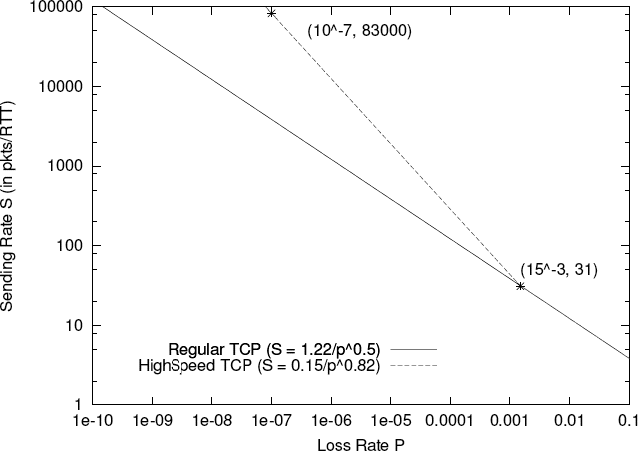
\includegraphics[width=0.7\textwidth]{imgs/16/16-19.png}
	\caption{在高速 TCP 中,针对更低的丢包率和更大的窗口,TCP 响应函数需要做相应的调整,从而在高带宽延迟的网络中获得更大的吞吐量。图片来自 Sally Floyd 2003年3月在 IETF TWVWG的演讲}
\end{figure}

为了使TCP 实现上述响应函数,需要调整拥塞避免机制。当窗口发生改变时,需要考虑当前的窗口大小。与传统 TCP类似,在接收一个好的ACK 后需要参考当前窗口大小来调
整窗口值。具体响应如下:
\begin{equation}
    cwnd, + 1 = cwnd, + a (cwnd,) /cwnd,
\end{equation}
当对于拥塞事件进行响应时(例如丢包,或者发现ECN 标志),它的响应如下:
\begin{equation}
    cwnd, + 1 = cwnd, - b (cwnd,) * cwnd,
\end{equation}
这里的 a0 是和式增加函数,而b0 是积式减小函数。在标准TCP 中,它们都是当前窗口大小的相关函数。为了获得预期的响应函数,我们首先由公式(16-3)推广得出以下公式:

变换得:
\begin{equation}
    a (w)=2P,M3b (w)/(2-b(w))
\end{equation}
上述关系式有多个解,也就是说,有多种a0 和b0的组合方式可以满足,然而有些解对于调度算法来说并不适用。

[RFC3649]中还给出了其他的 HSTCP 对传统 TCP 的拥塞避免改进的细节。[RFC3742]描述了如何修改慢启动阶段,使其在高速环境下得到运行中的拥塞窗口值。它被称为受限的
慢启动,即减慢速度的慢启动,这样在处理大窗口的情况下(几千甚至几万个数据包),TCP不会在一个 RTT 中使窗口翻倍。

在受限的慢启动阶段,引人了一个新的参数称为 \verb|max_ssthresh|。这个值不是 ssthresh 的最大值,而是 cwnd 的一个阈值:如果 \verb|cwnd < = max_ssthresh|,则慢启动阶段与传统 TCP 相
同。如果 \verb|max_ssthresh <cwnd <= ssthresh|,那么 cwnd 在每个RTT 中最大只能增长\verb|(max_ssthresh/2)| 个 SMSS。具体管理 cwnd的方式如下:
\begin{verbatim}
    if (cwnd <= max_ssthresh) /
wnd = cwnd + SMSS
(regular slow start)
y else {
K = int (cwnd / (0.5 * max_ssthresh) )
cwnd = cwnd + int ( (1/K) *SMSS)
(limited slow start)
\end{verbatim}
建议 \verb|max_ssthresh| 的初始值为100个包,或者 100*SMSS个字节。

\subsection{二进制增长拥塞控制(BIC和 CUBIC)}
HSTCP 是为在大BDP 网络中实现高吞吐量的一种 TCP 修改方案。它兼顾了在普通环境下与传统 TCP 的公平性,但在特环境中能够达到更快的发送速度。在多个具有不同 RTT
的连接竞争带宽时,HSTCP 不会直接控制这些竞争行为(称为“RTT 公平性”)。对标准TCP的研究表明,当使用相同的数据包大小和 ACK策略时,较小的 RTT 在共享传输路径上
能获得更大的带宽[F91]。对于能根据自身窗口大小来调节 cwnd 增长值的TCP(称力帶宽可扩展TCP)来说,这种不公平性表现得更加严重。是否遵守 RTT公平性一直是一个存在争论
的话题。尽管第一感觉认为 RTT公平性是必要的,但是拥有较大 RTT 的连接可能会使用更多的网络资源(例如经过更多的路由器),所以拥有较小的吞吐量也是合理的。不论是哪种观
点,了解 RTT的公平性(或不公平性)行为是我们接下来探讨各个 TCP改进版本的动因。

\subsubsection{BIC-TCP 算法}
为建立一种可扩展的TCP及解决RTT公平性问题,提出了BIC-TCP 算法(之前称为BI-TCP 算法)[XHR04],并从Linux 2.6.8 内核版本中开始应用。BIC TCP 算法的主要目的
在于,即使在拥塞窗口非常大的情况下(需要使用高带宽的连接),也能满足线性 RTT公平性(linear RTT fairness)。线性 RTT公平性是指连接得到的带宽与其 RTT成反比,而不是一
些更复杂的函数。

该方法使用了两种算法来修改标准 TCP 发送端:二分搜索增大(binary search increase)和加法增大(additive increase)。这些算法在出现一个拥塞信号(如丢包)后被调用,但是在
任一给定时刻只运行一种算法。二分搜索增大算法的操作过程如下:当前最小窗口是最近一次在一个完整 RTT 中没有出现丢包的窗口大小,最大窗口是最近一次出现丢包时的窗口大
小。预期窗口位于这两个值之间。BIC-TCP 使用二分搜索技术选择这两个值的中点作为一个试验的窗口,然后进行递归。如果这个点依然会发生丢包,那么将它设置为最大窗口,然后
继续重复上述过程。如果不发生丢包,那么将它设置为新的最小窗口,然后同样继续重复上述过程。直到最大窗口和最小窗口的差值小于一个预先设置好的阈值时,这一过程才停止,
其中这个阈值被称力最小增量(minimum increment),或者 Smino

这一算法往往会在一个对数级的试验次数内找到预期窗口,也被称为饱和点(saturationpoint)。而标准 TCP 则需要多项式级的次数(平均为窗口大小差值的一半)。因此,这种方法
使BIC-TCP 在特定的处理阶段拥有比标准 TCP 更快的速度。它是为充分利用高速网络没有不必要延时的优点而设计的。与其他协议相比较,BIC-TCP 表现得有所不同,它的增长速率
在一些时间点是下降的,也就是说,越接近饱和点,它增长得越慢。而大多数其他算法在接近饱和点时都会增长得更快。

加法增大算法运作过程如下:当使用二分搜索增大算法时,可能会出现当前窗口大小与中间点(从二分搜索意义上说)之间差距很大。由于可能出现突然大量数据注入网络的情
况,所以在一个 RTT 内将窗口增大到中间点可能并不是一个好方法。这种情况下就要采用加法增大算法。当中间点与当前窗口大小之间的差值大于一个特定值 Smox的时候,将调用
加法增大算法。此时,增量被限制为每个 RTT增加 SIhx,这一增量被称为窗口夹(windonclamping)。一旦中间点距离试验窗口比距离Smux值更近时,则转换为使用二分搜索增大算
法。总的来说,当检测到丢包现象,窗口会使用乘法系数B来减小,而窗口增大时,首先使用加法增大算法,之后一旦确认加法增量小于 Smox 时就转为使用二分搜索增大算法。这种生
合的算法称为二进制增长 (binary increase),或者 BI。

当窗口增至超过当前最大值,或由于还没有丢包发生而没有已知的最大值时,增长会终止。这是由最大位探测(max probing)机制所实现的。最大值探测的目的是有效地利用带宽。
它使用一种加法增大和二分搜索增大的对称方式。初始时,它设置了一个较小的增量。之后如果没有检测到拥塞,它就会使用更大的增量。因为在饱和点附近变化量较小,而且在饱和
点处网络能够表现出最佳的性能,所以这种方法具有良好的稳定性。

Linux 系统(内核版本2.6.8至2.6.17)中实现了BIC-TCP 算法,并默认开启。有4个系统参数用来控制它的操作:\verb|net.ipv4.tcp_bic|、\verb|net.ipv4.tcp_bic_beta|、\verb|net.ipv4.tcp_bic_low_window|
和 \verb|net.ipv4.top_bic_fast_convergence|。第一个布尔变量用来控制是否使用BIC(与传统的快速重传和快速恢复相对应)。第二个变量包含了一个比例因子,它可以通过cwnd 值来决定Smut 值
(默认为 819)。第三个参数控制在运行 BIC-TCP算法前的最小拥塞窗口的大小。它的默认值为14,这意味着标准 TCP 拥塞控制决定最小窗口。最后一个参数是一个标志位,默认状
态下是开启的。在二分搜索增大算法处于下降趋势时,它会影响新的最大窗口和目标窗口的选择。在窗口减小的过程中,新的最大窗口和最小窗口将被分别设置cwnd 和一定比例的
cwnd 值(由参数B决定,即B*cwnd)。如果启用快速收敛,并且新的最大值小于它之前的值,那么最大窗口将在它与最小窗口的平均值范围内继续减小。在这之后,不论快速收敛是
否开启,目标窗口将设置为最大窗口与最小窗口的平均值。这种方式有助于在多个 BIC-TCP流共享一个路由器时,更快地分配带宽。

\subsubsection{CUBIC}
BIC-TCP 的开发者对基本算法进行改进,形成新的控制算法,称 CUBIC [HRX08]。自2.6.18 内核版本起,它一直是Linux 系统的默认拥塞控制算法。CUBIC 改进了 BIC-TCP
在一些情况下增长过快的不足,并对窗口增长机制进行了简化。它不像 BIC-TCP 那样使用阈值(Smux)来决定何时调用加法增大算法和二分搜索增大算法,而是使用一个高阶多项式
函数(具体来说是一个三次方程)来控制窗口的增大。三次方程的曲线既有凸的部分也有凹的部分。这就意味着,在一些部分(凹的部分)增长比较缓慢,而在另一些部分(凸的部分)
增长比较迅速。在BIC 算法和 CUBIC 算法之前,所有 TCP 研究提出的都是凸的窗口增长函数。CUBIC算法中,这个特殊的窗口增长函数如下所示:
\begin{equation}
    W(t)=C(t-K)’+Waax
\end{equation}

在这个表达式中,W (t)代表在时刻!的窗口大小,C是一个常量(默认为 0.4),t是距离最近的一次窗口减小所经过的时间,以秒为单位。K是在没有丢包的情况下窗口从W增长
到 Waux所用的时间。Wmux是最后一次调整前的窗口大小。其中K可依据以下表达式计算:

其中B是积式减少的常量(歌认为0.2)。图16-20为K=2.71、Wmm =10、C=0.4时,在时间段为t=10,5]时 CUBIC 窗口增大算法的图示。

图中显示了 CUBIC窗口增大函数既包含凸的部分也包含凹的部分,当发生快速重传时,Wm被设置为 ewnd,新的 cwnd 值和 ssthresh 值被设置为B* cwnd。 CUBIC 算法中的B
默认为0.8。I (+ RTT)值是下一个目标窗口的值。当在拥塞避免阶段,每收到一个ACK,cwnd 值增加(W(t+ RTT) - cwnd)/cwnd。

值得注意的是,将t设置为距上次窗口减小经过的时间,有助于确保RTT的公平性。这里并不使用固定值对窗口进行改变,而用关于,的函数来调节窗口大小。这种方法将窗口变
更操作从传统模式中分离出来。

\begin{figure}[!htb]
    \centering
	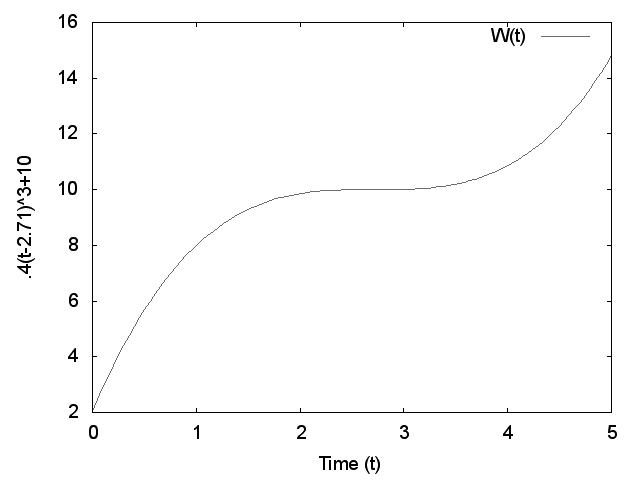
\includegraphics[width=0.7\textwidth]{imgs/16/16-20.png}
	\caption{CUBIC 窗口增长函数是一个关于的三次函数。它在W (4)<Wmax 的区域是凹函数。在这一区域,cwnd 的增长越来越慢。在达到Wa之后,增长函数变为凸函数。在这一区域。cwnd
        的增长越来越快}
\end{figure}

除了三次方程之外,CUBIC还有“TCP 友好”策略。当窗口太小使得 CUBIC 不能获得比传统 TCP 更好的性能时,它将会开始工作。根据1可以得到标准 TCP 的窗日大小 Tep (A):

当在拥塞避免阶段有一个ACK 到达时,如果 cwnd 值小于 Wep (①),那么 CUBIC 将 cwnd 值设置为 Wop(①)。这种方法确保了 CUBIC在一般的中低速网络中的TCP 友好性,而在这些网
络中标准 TCP 相对CUBIC算法更具优势。

如前所述,从 Linux 2.6.18 内核版本起,CUBIC 算法就是 Linux 系统的默认拥塞控制算法。而从2.6.13版开始,Linux 支持可装卸的拥塞避免模块[PO7],用户可以选择想用的算法。
变量 \verb|net.ipv4.tcp_congestion_control| 表示当前默认的拥塞控制算法(默认为 cubic)。变量 \verb|net.Ipv4.tep_available _congestion_control| 表示系统所载人的拥塞控制算法(一般,其他的算法可
被作为内核模块载人)。变量 \verb|net.jpv4.top_allowed congestion_ control| 表示用户允许应用程序使用的算法(可以具体选择或者设为默认)。它默认支持 CUBIC 算法和Reno算法。

\section{基于延迟的拥塞控制算法}
前面介绍的拥塞控制方法都是通过检测丢包、利用一些 ACK 或SACK 报文探测、ECN算法(如果可用)、重传计时器的超时来触发的。ECN 算法(16.11 节)允许一个 TCP发送
端向网络报告拥塞状况,而不用检测丢包。但是这要求网络中每一个路由器的参与,比较难以实现。然而,在没有ECN 的情况下,判断网络中的主机是否发生拥塞也是可能的。当
发送端不断地向网络中发送数据包时,不断增长的RTT值就可以作为拥塞形成的信号。我们在图 16-8中看到过这种情况。新到达的数据包没有被发送,而是进入等待队列,这就造
成了 RTT值不断增大(直到数据包最终被丢弃)。一些拥塞控制技术就是根据这种情况提出的。它们被称为基于延迟的拥塞控制算法,与我们至今为止看到的基于丢包的拥塞控制算
法相对。

\subsection{Vegas 算法}
TCP Vegas 算法于1994年被提出[BP95]。它是TCP 协议发布后的第一个基于延迟的拥塞控制方法,并经过了TCP协议开发组的测试。Vegas 算法首先估算了一定时间内网络能够
传输的数据量,然后与实际传输能力进行比较。若本该传输的数据并没有被传输,那么它有可能被链路上的某个路由器挂起。如果这种情况持续不断地发生,那么 Vegas发送端将降低
发送速率。这与标准 TCP 中利用丢包来判断是否发生拥塞的方法相对。

在拥塞避免阶段,Vegas 算法测量每个 RTT 中所传输的数据量,并将这个数除以网络中观察到的最小延迟时间。算法维护了两个阈值a和B(a小于B)。当吞吐量(窗口大小除以
观察到的最小 RTT)与预期不同时,若得到的吞吐量小于Q,则将拥塞窗口增大;若吞吐量大于B,则将拥塞窗口减小。吞吐量在两阈值之间时,拥塞窗口保持不变。拥塞窗口所有的
改变都是线性的,这意味着这种方法是一种和式增加/ 和式减少(Additive Increase/AdditiveDecrease, AIAD)的拥塞控制策略。

作者通过链路瓶颈处的缓冲区利用率来描述 a和B。a 和B的最小值分别设置为1和3。设置该值的原因是:在网络中至少有一个数据包缓冲区会被占用(也就是说,路由器上的队
列表示网络链路上的最小带宽)才能保持网络资源被充分利用。如果 Vegas 只维护一个缓冲区,那么当有其他可用带宽时,就要等待额外的 RTT时间。因此为了传输更多的数据,需
要多使用两个缓冲区(达到3,a的值)。此外,保持一个区间(B-a)可以保留一部分空间,使得吞吐量可以有小幅改变而不至引发窗口大小的改变。这种缓冲机制可以减少网络的震荡。

稍加修改后,这种方法也适用于慢启动阶段。这里,每隔一个 RTT, cwnd 值才随着一个好的ACK 响应而加1。对于cwnd没有增长的RTT,需要测量吞吐量是否在增长。如果没
有,发送端将转为 Vegas 拥塞避免方式。

在特定情况下,Vegas 算法会盲目地相信前向的延迟会高于它实际的值。这种情况发生在它相反的方向产生了拥塞(回忆一下,TCP 连接的两个方向的链路可能会不同,并产生不
同程度的拥塞状态)。在这种情况下,虽然不是发送端导致了(反向的)拥塞,但是返回发送端的数据包(ACK)会产生延迟。这就使得在这种不是真正需要调整拥塞窗口的情况下,
减小了窗口大小。这是大多数基于测量 RTT来进行拥塞控制判断的方法所共有的潜在缺陷。甚至,在反方向上严重的拥塞问题会导致 ACK 时钟(图16-1)的严重紊乱[M92]。

Vegas 与其他的 Vegas TCP 连接平等共用一条链路,因为每一次向网络中传输的数据量都很小。然而,Vegas 与标准 TCP 流共用链路时则是不平等的。标准 TCP 的发送端想要占
满网络中的等待队列,反之 Vegas 则是想使它们保持空闲。因此,当标准 TCP 发送端发送数据包时,Vegas发送端会发现延迟在增长,那么它就会降低发送速率。最终,这导致了只对
标准 TCP 有利的状态。Linux 系统支持 Vegas,但不是默认开启的。对于2.6.13 之前的内核版本来说,布尔型 sysetl 变量 \verb|net.ipv4.top_vegas_cong_avoid| 决定了是否使用 Vegas (默认为
0)。变量 \verb|net.ipv4.top_vegas_alpha|(默认为2)和变量 \verb|net.jpv4.top_vegas_beta|(默认为6)决定了上面提到的a和B值,但是它们的单位是半个数据包(也就是说,6对应着3个数据包)。
变量 \verb|net.ipv4.tcp_vegas_gamma|(默认为 2)用于配置在经过多少个半数据包后 Vegas 结束慢启动阶段。对于2.6.13之后的内核版本,Vegas 需要作为分离的内核模块被载人,通过设置
\verb|net.ipv4.tcp_congestion_control| 来启动 vegas。

\subsection{FAST 算法}
FAST TCP 算法是为处理大带宽延迟的高速网络环境下的拥塞问题而提出的[WJLH06]。原理上与Vegas 算法相同,它依据预期的吞吐量和实际的吞吐量的不同来调整窗口。与
Vegas 算法不同的是,它不仅依据窗口大小,而且还依据当前性能与预期值的不同来调整窗口。FAST 算法会使用速率起搏 (rate-pacing)技术每隔一个 RTT 都会更新发送率。如果测量
延迟远小于阈值时,窗口会进行较快增长,一段时间后会逐渐平缓增长。当延迟增大时则相反。FAST 算法与我们之前所说的方法不同,因为在其中包含了一些专利,并且它正被独立
地商业化。FAST 算法被一些研究机构质疑缺乏安全性,但是一个评估报告[S09]显示它具有良好的稳定性和公平性。

\subsection{TCP Westwood 算法和 Westwood+算法}
TCP Westwood 算法(TCPW)和 TCP Westwood +算法(TCPW +)的设计目的在于,通过修改传统的 TCP NewReno 发送端来实现对大带宽延迟积链路的处理。TCPW +算法是对
TCPW 算法的修正,所以这里只对 TCPW 算法进行说明。在TCPW 算法中,发送端的合格这率估计(ERE)是一种对连接中可用带宽的估计。类似 Vegas 算法(基于预期速率与实际
速率的差别),该估计值被不断计算。但是不同的是,对于这个速率的测量会有一个测量间隔,该间隔基于ACK 的到达动态可变。当拥塞现象不明显时,测量间隔会比较小,反之亦
然。当检测到一个数据包丢失的时候,TCPW不会将cwnd值减半,而是计算一个估计的BDP 值(ERE 乘以观察到的最小 RTT),并将这个值作为新的ssthresh 值。另一方面,在连
接处于慢启动阶段时,使用一种灵活的探测机制(Agile Probing)[WYSGOS]适应性地反复设置 ssthresh 值。因此当 ssthresh 值增长时(由于初始的慢启动),cwnd值会以指数形式增长。
在Linux 2.6.13之后的内核版本中,可以通过加载一个TCPW模块,并设置\verb|net.ipv4.tcp_congestion_control| 为 Westwood 来启动 Westwood。

\subsection{复合TCP}
类似于 Linux 系统中的可装卸的拥塞避免模块,从 Windows Vista 系统开始,用户也可以自主选择使用何种 TCP 拥塞控制算法。该选项(除了 Windows Server 2008外,默认不开
肩)称为复合 TCP (Compound TCP,CTCP)[TSZS06]。CTCP 不仅依据丢包来进行窗口的调整,还依据延迟的大小。可以认为它是一种标准 TCP 和 Vegas算法的结合,而且还包含了
HSTCP 可扩展的特点。

Vegas 算法和 FAST 算法的研究结果显示,基于延迟的拥塞控制方法可以得到更好的利用率、更少的自诱导的丢包率、更快的收敛性(对于正确的操作来说),并且使RTT 更具公
平性和稳定性。然而,就像前面提到过的,基于延迟的方法在与基于丢包的拥塞控制方法竞争时会失去优势。CTCP 就是希望通过将基于延迟的方法和基于丢包的方法相结合来解决该
问题。为了达到这一目的,CTCP定义了一个新的窗口控制变量 dwnd(“延迟窗口”)。可用窗口大小™则变成了
\begin{equation}
    W = min (cwnd + dwnd, awnd)
\end{equation}

对cwnd值的处理与标准TCP 类似,但是如果延迟允许,新加入的dwnd 值会允许额外的数据包发送。在拥塞避免阶段当 ACK 报文到达时,cwnd 值根据下面的公式进行更新:
\begin{equation}
    cwnd = cwnd + 1/ (cwnd + dwnd)
\end{equation}
dwnd 值的控制是基于 Vegas 算法的,并且只在拥塞避免阶段才是非零值(CTCP 使用传统的慢启动方式)。当连接建立时,使用一个变量 baseRTT 来表示测量到的最小 RTT 值。然
后预期数据与实际数据的差值 diff 将使用如下公式进行计算:diff= *(1-(baseRTT/RTT))。其中 RTT 是估算的(平滑的)RTT估计。diff的值估算了网络队列中的数据包数量(或字节
数)。与大多数基于延迟的方法类似,CTCP 算法试图将 diff 值保持在一个阈值内,以此保证网络的充分利用而不至于出现拥塞,这个阈值定义为y。为了达到这一目的,对于dwnd值
的控制可依据以下公式:

其中(x)*表示 max (x, 0)。注意这里 dwnd 值非负。而当 CTCP 像标准TCP 那样工作的时候,dwnd 值应为0。

在第一种情况下,网络没有被充分利用,CTCP 根据多项式a*win(d)'增大 dwnd值。这是一种多项式级的增长,而当缓冲区的占用率小于y时,会更快速地增长(类似于
HSTCP)。在第二种情况下,缓冲区的占用率已经超过了阈值y,固定值6表示延迟窗口的递减速率(dwnd经常为cwnd 的加数)。这就使得CTCP 的RTT更具公平性。当检测到丢包时,
dwnd 值会有自己的积式递减系数B。

可以看到,CTCP需要使用参数K、a、B、》和5。k的值表示速度的等级。与HSTCP类似,可以将k值设置为0.8,但是由于实现方面的原因,k值被设置为0.75。a 和B值表示了
平滑度和响应性,分别被默认设置为0.125和0.5。对于》值,这里凭借经验将其设置为30个数据包。如果这个值太小,将不会有足够的数据包,以致不能得到较容易测量的延迟。相
反,如果这个值太大则会导致长时间的拥塞。

CTCP 算法相对比较新,通过更深人的实验和改进,会使其与标准 TCP 相比拥有更好的性能,并且能够很好地适应不同的带宽。在一个仿真实验中,[W08] 注意到在网络缓冲区较
小时(小于》值),CTCP 算法的性能会很差。他们还提出 CTCP 也存在着一些 Vegas 算法中的问题,包括重新路由问题(适应具有不同延迟的新链路)和持续的拥塞问题。他们发现,
如果有很多的CTCP 流,其中每一个都要维护y个数据包,并且共用一条相同瓶颈的链路时,CTCP 的性能会非常差。

像前面所提到的,CTCP 在大多数版本的Windows 系统中不是默认开启的。然而,下面的命令可以用来选择 CTCP 作为拥塞控制方法。

\begin{verbatim}
    C: \> netsh interface top set global congestionprovider=ctep
\end{verbatim}

它可以通过另选一个不同的(或不设置)控制算法来关闭。CTCP 也作为一个可装卸式的拥塞避免模块而移植到 Linux 系统中,当然它也不是默认启用的。

\section{缓冲区膨胀}
虽然存储单元的价格昂贵(高端路由器也是如此),但是现在的网络设备中仍包含大量的内存和几百万字节的包缓冲区。然而,这样庞大的内存(与传统的网络设备相比)会导致
像TCP这样的协议性能下降。这一问题被称为缓冲区膨胀[G11][DHGSOT]。它主要存在于家用网关的上行端以及家庭或小型办公室的接人点处,与排队等待而产生的大量延迟有关。
标准 TCP 协议的拥塞控制算法会在链路的瓶颈处将缓冲区填满。而由于拥塞的信号(一个数据包丢失)需经很长时间才能反馈到发送端,此时在发送端和接收端之间缓存了大量数据,
TCP协议也不能很好地运作。

KWNP10] 中指出,在美国包括电缆和 DSL 在内,上传带宽范围是256Kb/s ~4Mb/S,在商用路由器上的缓冲区大小应该在16KB 至256KB 之间。图16-21 显示了在几种缓冲区大
小下延迟和数据传输速率的关系,可以证明之前结论的正确性。


\begin{figure}[!htb]
    \centering
	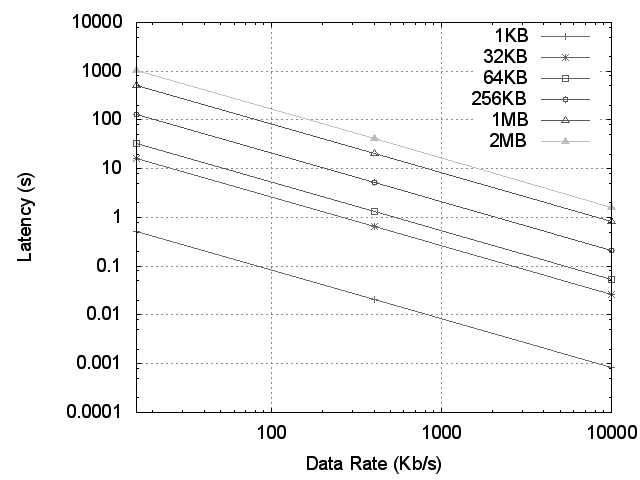
\includegraphics[width=0.7\textwidth]{imgs/16/16-21.png}
	\caption{双对数坐标系显示了队列等待的延迟随拥塞队列长度的变化情况。当缓冲区被占满时(“缓冲区膨胀”),交互式的应用程序将会产生无法容忍的延迟}
\end{figure}

图16-21展示了针对不同缓冲区大小(1KB ~2MB)数据在队列等待所产生的延迟情况。如果缓冲区大小为几百 KB 或者更多,那么家庭网络上传带宽速率(一般在250Kb/s至
10Mb/s之间)会引起几百秒的延迟。为了给用户带来更好的体验,一般的交互式应用程序需要把单向延迟控制在 150ms 以下[G114]。因此,如果缓冲区被一个或多个大的上传文件所
占满(如BT共享文件),会严重影响交互式应用性能。

不是所有的网络设备中都存在缓冲区膨胀的问题。实际上,主要问题是缓冲区端用户接人设备过满。有很多方法可以解决这一问题,包括修改协议(如像 Vegas 这样的基于延迟的
拥塞控制方式,但是它可能会因为网络抖动而产生相反效果 [DHGSO7)、使用缓冲区大小可动态改变的接人设备([K WNP10] 中提到),或将两者结合。接下来介绍一种综合的方法,它
不仅可以解决缓冲区膨胀的问题,而且还有一些其他的好处。

\section{积极队列管理和 ECN}
到现在为止,TCP能够推断出拥塞产生的唯一方法就是发生丢包现象。特别是路由器(最有可能产生拥塞)通常不会通知连接两端的主机,TCP 即将产生拥塞。而是当缓存没有
多余的可用空间时,只好将新到达的数据包丢弃(称为“尾部丢弃”)。然后依照先进先出(FIFO)的方法继续转发那些先前到达的数据包。当网络路由器像这样被动工作时(指它们
在超负荷的时候仅仅丢弃数据包,而不会提供它们已经处于拥塞状态的任何反馈信息),TCP除了事后再做出反应以外无能为力。然而,如果路由器可以更积极地管理它们的等待队列
(也就是说使用更精确复杂的调度算法和级存管理策略),也许这种情况就能得到改善。若可以将拥塞状态报告给端节点,效果会更好。

应用 FIFO 和尾部丢弃以外的调度算法和缓存管理策略被认为是积极的,路由器用来管理队列的相应方法称为积极队列管理((AQM)机制。[RFC2309]中提到了AQM 机制的潜在
优势。若可以通过将路由器和交换机的状态传输给端系统来实现 AQM 时,它将更具利用价值。这些在TRFC3168] 中有详细描述,[RFC3540]利用相关实验描述了扩展安全性的 AQM。
这些 RFC 都描述了显式拥塞通知(Explicit Congestion Notification, ECN),它对经过路由器的数据包进行标记(设置 IP 头中的两个 ECN 标志位),以此得到拥塞状况。

随机早期检测(RED)网关[FJ93]机制能够探测拥塞情况的发生,并且控制数据包标记。这些网关实现了一种衡量平均占用时间的队列管理方法。如果占用队列的时间超过最小
值(minthresh),并且小于最大值(maxthresh),那么这个数据包将被标记上一个不断增长的概率值。如果平均队列占用时间超过了 maxthresh,数据包将被标记一个可配置的最大的概
率值(MaxP),MaxP 可以设置为1.0。RED 也可以将数据包丢弃而不是标记它们。

\begin{tcolorbox}
    RED 算法有多种版本(如思科的 WRED 就是基于IP DSCP 和优先级的 RED算法),很多路由器和交换机都支持。
\end{tcolorbox}

当数据包被接收时,其中的拥塞标记表明这个包经过了一个拥塞的路由器。当然,发送端(而不是接收端)才真正需要这些信息,以此降低发送速率。因此,接收端通过向发送端
返回一个 ACK 数据包来通知拥塞状况。

ECN机制主要在 IP层进行操作,也可以应用于 TCP 协议之外的其他传输层协议。当一个包含ECN 功能的路由器经过长时间的拥塞,接收到一个 IP 数据包后,它会查看 IP 头中的
ECN 传输能力(ECT)标识(在I头中由两位 ECN 标志位定义)。如果有效,负责发送数据包的传输层协议将开启 ECN 功能,此时,路由器会在IP头设置一个已发生拥塞(CE)标识
(将ECN 位都置为1),然后继续向下转发数据报。若拥塞情况不会持续很长时间(例如由于队列溢出导致最新的一个数据包被丢弃),路由器不会将CE 标识置位。因为即使是一个单独
的CE 标识,传输协议也会做出反应。

如果 TCP接收端发现接收到的数据包的 CE标识被置位,那么它必须将该标识发送回发送端([RFCSS62]中的实验表明,也可以将ECN添加到 SYN+ACK报文段中发送)。因为
接收端经常会通过 ACK 数据包(不可靠的)向发送端返回信息,所以拥塞标识很有可能会丢失。出于对这种情况的考虑,TCP 实现了一个小型的可靠连接协议,通过这个协议可以将标
识返回给发送端。TCP接收端接收到 CE 标识被置位的数据包之后,它会将每一个ACK 数据包的“ECN回显”(ECN-Echo)位字段置位,直到接收到一个从安送瑞发来的CWR 位字
段设置为1的数据包。CWR位字段被置位说明拥塞窗口(也就是发送速率)已经降低。

\begin{equation}
    RED 机制和ECN 机制至今已有将近20年,它们仍无法滿足广泛应用的网络调度。多种原因造成了此种现状(例如,RED 参数难以设置,而且能起的作用也
    有限)。2005年,对于ECN的“复畫”[KOS] 指出,只在数据包中应用ECN机制大幅限制了它的作用。[RFCSS62]中的一个实验表明,在一定负载下(例如Web流
    量),将ECN 放置在SYN+ACK 数据包中传输可以提高 ECN的实用性。
\end{equation}

TCP发送端接收到含有 ECN-Echo标识的ACK 数据包时,会与探测到单个数据包丢失时一样调整cwnd 值。同时发送端还会重新设置后续数据包的CWR位字段。常规的拥塞处
理方式为:调用快速重传和快速恢复算法(当然,数据包不会进行重传),这样就可以使TCP在丢包之前降低发送速率。值得注意的是,TCP 的处理不应该过度。特别是它不能对同一个
数据进行多次响应。否则,ECN TCP 相对于其他来说会处于不利地位。

在 Windows Vista 及之后的版本中,激活ECN 功能需要使用以下命令:
\begin{equation}
    C: \> netsh int tep set global encapability=enabled
\end{equation}

在 Linux 系统中,如果布尔型 Sysctl 变量 \verb|net.jpv4.tcp_ecn| 的值非零,则ECN 功能被微活。这种基于 Linux 的改变默认设置的方法正在广泛使用。在 Mac OS 10.5 及更新的版本中,
变量 \verb|net.inet.top.ecn_initiate_out| 和 \verb|net.inet.tcp.ecn_negotiate_in| 分别控制向外传输和向内传输的ECN功能的开启。当然,没有路由器和交换机的协作,ECN 的实用性在任何情况下都
会受到限制。AQM 在整个全球互联网络中发挥作用还需要时间。

\begin{tcolorbox}
    由于设计目的不同,RED机制和ECN机制被用于完全不同的操作环。Microsoft 和 Stanford 开发了 Data Center TCP (DCTCP)[A10]。它使用了更简化的
    参数,在第2层交换机上实现了 RED机制,可以在网络产生瞬时的拥塞时对数据包进行标记。它们还调整了 TCP接收端的行沟,只有在最后一个接收到的数据包包含
    CE 标记时,才将ACK 中的ECN-Echo 标记置位。报告显示达到相同的TCP 吞吐量情况下,缓冲区的占用率下降了90\%,并使背景流量增长10倍。
\end{tcolorbox}

\section{与TCP 拥塞控制相关的攻击}
我们已经看到生成数据包是如何攻击 TCP,使其改变自身的连接状态机,从而断开连接的。当 TCP 处于 ESTABLISHED 状态时,它也会受到攻击(至少为非正常工作状态)。大多
数针对 TCP拥塞控制的攻击都是试图强迫 TCP发送速度比一般情况更快或者更慢。

更早期的攻击方式是利用ICMPv4 Source Quench(源抑制)报文的结构。当这些报文被发送到运行 TCP协议的主机上时,任何与该 IP 地址相连的连接都会减慢发送速率。该1地
址包含在 ICMP 报文中的违规数据报中。然而随着 1995年路由器不再使用 Source Quench报文进行拥塞控制([RFC181215.:3.6 节),这种攻击方式也变得不可行了。另一方面,对于终端
主机,[RFC1122]规定 TCP 针对 Source Quench报文必须降低速率。综合以上两点,解决这种攻击最简单的方法就是在路由器和主机上阻止ICMP Source Quench 报文的传输。这种方
式已得到普遍使用。

一种更复杂、更常用的攻击方式是基于接收端的不当行为[SCWA99]。这里将描述三种攻击形式,它们都可以使TCP发送端以一个比正常状态更快的速率进行数据发送。这些攻
击可用于使某个 web 客户端得到比其他客户端更高的优先权,分别为ACK分割攻击、重复ACK欺骗攻击、乐观响应攻击,还有一种在TCP 中实现的变体,这里把它称为“TCP
Daytona"。

ACK 分割攻击的原理是,将原有的确认字节范围拆分成多个ACK 信号并返回给发送端。由于TCP 拥塞控制是基于 ACK 数据包的到达进行操作的(而不是依据ACK 信号中的
ACK 字段)。这样发送端的cwnd 会比正常情况更快速地增长。要解决这一问题,与ABC(适当字节数)类似,可通过计算每个 ACK 能确认的数据量(而不是一个数据包的到达)来判断
是否力真的 ACK。

重复ACK 欺骗攻击可以使发送端在快速恢复阶段增长它的拥塞窗口。回想之前讨论过的,在标准快速恢复模式中,每次接收到重复 ACK cwnd 都会增长。这种攻击会比正常情况
更快地生成多余的重复ACK。因为还没有一种明确的方法可以将接收到的重复 ACK 和它们所确认的报文段相对应(一个基于时间的伪随机数可以解决这一问题,我们将在第18章详
细讨论),因此这种攻击更加难以防治。利用时间戳选项可以解决这一问题,可以设置该选项在每个连接中开启或关闭。然而解决这一问题的最好方法是,限制发送端在恢复阶段的在
外数据值。

乐观响应攻击原理是对那些还没有到达的报文段产生ACK。因为TCP 的拥塞控制计算是基于端到端的RTT的。对那些还没有到达的数据提前进行确认就会导致发送端计算出的
RTT 比实际值要小,所以发送端将会比正常情况下更快地做出反应。但如果发送端接收到了一个未发送数据的ACK,通常会选择忽略该响应。与其他攻击方式不同,这种方法不能在
TCP 层保证数据的可靠传输(也就是说,已经被确认的数据可能会丢失)。丢失的数据会被应用层或者会话层协议重建,这是很常见的(例如在 HTTP/1.1 中)。为防范这类攻击,可定
义一个可累加的随机数,使得发送数据段大小可随时间动态改变,以此来更好地匹配数据段和它对应的ACK。当发现得到的ACK 和数据段不匹配时,发送端就可以采取相应的行动。

接收端异常行为的问题也受到了一些研究ECN 的专家的关注,回想一下使用 ECN的AQM 机制,TCP 接收端会在 ACK 消息中向发送端返回一个 ECN标识。然后发送端据此将
会降低它的发送速率。如果接收端不能向发送端返回 ECN 标识(或者网络中的路由器将这一标识清除),那么发送端将不会知道是否产生拥塞,也就不会降低发送速率。[RFC3540]进行
了相关实验,即将一个 IP 数据包中的ECN 字段(2比特)中的ECT 位字段设置为随机数。发送方将该字段值设置为一个随机的二进制数,接收方将该字段的值加1(一个异或操作)。
当生成 ACK 响应时,接收端会把该值放置到TCP 头部的第7位(一般保留为0)。行异常的接收端有一半的概率可以猜到这一数值。因为每一个数据包都是相对独立的,所以一个行
为异常的接收端必须猪对每一个ECT 值,这样对于k个数据包来说全部猜对的概率只有1/2(对于任何一个长时间使用的连接这都是很微小的)。

\section{总结}
TCP被设计为互联网中主要的可靠传输协议。虽然其最初的设计包含了流量控制功能,能够在接收方无法跟上时降低发送方的速度,但是最初并没有提供方法从防止发送方淹没双
方之间的网络。在20世纪80年代末期,为了控制发送方的攻击性行为,TCP开发了慢启动与拥塞避免算法,从而避免了因网络拥塞而造成的丢包问题。这些算法都依赖于使用一个隐
含的信号、数据包丢失以及拥塞的指示。当检测到丢包时就会触发这些算法,无论是通过快速重传算法还是超时重传。

慢启动与拥塞避免通过在发送方设置一个拥塞窗口来实现对其操作的控制。该拥塞窗口将与传统的窗口一起使用(基于接收方提供的窗口广告)。一个标准的 TCP 会将其窗口的最
小值限定为2。随着时间的增长,慢启动要求拥塞窗口的数值指数地增加,而拥塞避免则会随着时间的推移而线性增长。在任何时刻都只能选择两种算法中的一种运行,而做出这一选
择则需要比较拥塞窗口当前的数值与慢启动的阈值。如果拥塞窗口超过了阈值,那么采用拥塞避免;否则使用慢启动。慢启动起初只在建立 TCP 逢接以及因超时而重新启动后使用。這
也适用于连接长时间处于空闲状态的情况。在整个连接的过程中,慢启动的阈值会动态地进行调整。

多年来,拥塞控制已经成为网络研究界关注的重要焦点之一。在通过 TCP与它的慢启动、拥塞避免过程获得经验后,一些改进方法被提出、执行以及标准化。通过跟踪 TCP 何
时从一系列丢包中恢复,NewReno(TCP 的一个改进版本)能够避免当多个数据包在同一个窗口中被丢弃时伴随 Reno变异发生的停滞现象。SACK TCP 通过允许发送者在一个 RTT中
智能地修复多个数据包改善NewReno的性能。在使用SACK TCP 时,需要仔细地核算,以确保发送者在与共享同一个互联网路径的其他TCP 通信方比较时不会显得过分积极。

近期,关于TCP拥塞管理的一些修改包括:速率减半、拥塞窗口的验证与调制,以及“撤销”过程。速率减半算法能够在检测出丢包后使拥塞窗口逐步而不是快速地减小。拥塞
窗口验证尝试在发送应用程序空闲或不能发送的情况下确保拥塞窗口不会过大;拥塞窗口调制限制了在接收到单一ACK后作为响应的突发传输的大小。“撤销”过程,例如Eifel 响应
算法,在数据包丢失信号被认为是虚假以及使用若干技术进行条件检测时撤销对拥塞窗口的修改。在上述情况下,为了将减小拥塞窗口所带来的负面影响降至最低,恢复拥塞状态至其
对应条件优于减小拥塞窗口。

经过 TCP 有意义的实践,发现拥塞避免过程需要花费相当长的一段时间才能找到并利用额外的可用带宽资源。因此,大量关于“带宽可扩展”的建议成为TCP 修改的方向。一
个较为知名的版本(在IETF 中)是HSTCP。相比于传统的TCP 而言,它允许拥塞窗口在大数值且少有数据包丢失的情况下更加积极地增长。此外,还有一些建议,如 FAST 和 CTCP。
它们的窗口增长过程都是基于数据包丢失与延迟的测量。在Linux 系统上广泛部署的 BIC.TCP 与 CUBIC 算法使用了增长函数。该函数在某些区间呈凸形,而在另一些区间则呈凹形。
这样就能够支持在饱和点的小窗口变化,从而可能以对新的可用带宽的迟缓响应(但仍快于标准的 TCP)为代价来增强稳定性。

随着显式拥塞通知(ECN)规范的提出,TCP 与互联网路由器的运营做出了一个重大改变,即在出现丢包之前允许 TCP 检测是否开始发生拥塞。虽然模拟与研究的结果表明它
是可取的,但它需要适度地调整 TCP 的实现,并使互联网路由器的操作方式发生重要改变。这种能力将部署到何种程度还有待观察。

虽然TCP 提供了最广泛使用的互联网可靠数据传输方法,但是它并没有以自身的安全方式实现。一般来说,它非常容易受到伪造数据包攻击,从而导致连接中断;攻击者只需要
猜出一个可行的(窗口)序列号就能够发起上述攻击。此外,没有任何完全可行的方法能够阻止一个过分积极的发送者仅仅违反所有的拥塞控制规则。


将所有为 TCP 而开发的算法和技术都结合到一个 TCP实现中并非易事(Linux 2.6.38 的TCP/IPv4大约有20000行C语言代码),而分析真实世界中TCP活动的记录需要耗费时间。
诸如 tcpdump、Wireshark 以及 tcptrace这样的工具使这项工作变得相对容易。由于动态地适应网络性能,使用基于时间序列图的可视化技术能够更容易理解 TCP的行为,例如本章所
采用的例子。

\section{参考文献}
